%% 
%% Copyright 2007-2020 Elsevier Ltd
%% 
%% This file is part of the 'Elsarticle Bundle'.
%% ---------------------------------------------
%% 
%% It may be distributed under the conditions of the LaTeX Project Public
%% License, either version 1.2 of this license or (at your option) any
%% later version.  The latest version of this license is in
%%    http://www.latex-project.org/lppl.txt
%% and version 1.2 or later is part of all distributions of LaTeX
%% version 1999/12/01 or later.
%% 
%% The list of all files belonging to the 'Elsarticle Bundle' is
%% given in the file `manifest.txt'.
%% 
%% Template article for Elsevier's document class `elsarticle'
%% with harvard style bibliographic references

\documentclass[preprint,12pt,authoryear]{elsarticle}
\usepackage[margin=2.5cm]{geometry} % uniform 2.5 cm margin
%% Use the option review to obtain double line spacing
%% \documentclass[authoryear,preprint,review,12pt]{elsarticle}

%% Use the options 1p,twocolumn; 3p; 3p,twocolumn; 5p; or 5p,twocolumn
%% for a journal layout:
%% \documentclass[final,1p,times,authoryear]{elsarticle}
%% \documentclass[final,1p,times,twocolumn,authoryear]{elsarticle}
%% \documentclass[final,3p,times,authoryear]{elsarticle}
%% \documentclass[final,3p,times,twocolumn,authoryear]{elsarticle}
%% \documentclass[final,5p,times,authoryear]{elsarticle}
%% \documentclass[final,5p,times,twocolumn,authoryear]{elsarticle}

%% For including figures, graphicx.sty has been loaded in
%% elsarticle.cls. If you prefer to use the old commands
%% please give \usepackage{epsfig}

%% The amssymb package provides various useful mathematical symbols
\usepackage{amssymb}
%% Useful packages
\usepackage{tabularx}
\usepackage{booktabs}
\usepackage{tikz}
\usepackage{pgfplots}
\pgfplotsset{compat=1.18}
\usepackage{amsmath}
\usepackage{graphicx}
\usepackage{xcolor}
\usepackage[colorlinks=true, allcolors=blue]{hyperref}
\usepackage{caption}
\usepackage{subcaption}
\usepackage{sectsty}
\usepackage{float}
\usepackage{subfiles}
\usepackage{soul}

%% Toggle for the structured TODO overview page before the manuscript
%% Set to \showtodooverviewfalse before submission to hide the overview page
\newif\ifshowtodooverview
\showtodooverviewtrue

\DeclareRobustCommand{\todobacklink}{%
  \ifshowtodooverview\quad{\scriptsize\hyperlink{todo-overview}{[\,$\uparrow$ Overview\,]}}\fi
}

\newcommand{\timo}[1]{\todo[inline, color=orange!30]{\textbf{Timo:} #1\todobacklink}}
\newcommand{\leif}[1]{\todo[inline, color=yellow!40]{\textbf{Leif:} #1\todobacklink}}
\newcommand{\aitodo}[1]{\todo[inline, color=red!40]{\textbf{AI TODO:} #1\todobacklink}}
\newcommand{\yanetsi}[1]{\todo[inline, color=purple!40]{\textbf{Yanetsi:} #1\todobacklink}}
\newcommand{\RevieweroneRTBM}[1]{\todo[inline, color=green!40]{\textbf{Revier1RTBM:} #1\todobacklink}}
\newcommand{\alex}[1]{\todo[inline, color=blue!40]{\textbf{Alex:} #1\todobacklink}}

\newcommand{\todobadge}[2]{\colorbox{#1}{\textbf{\scriptsize #2}}}
\newcommand{\badgeTimo}{\todobadge{orange!30}{Timo}}
\newcommand{\badgeLeif}{\todobadge{yellow!40}{Leif}}
\newcommand{\badgeAlex}{\todobadge{blue!25}{Alex}}
\newcommand{\badgeYanetsi}{\todobadge{purple!30}{Yanetsi}}
\newcommand{\badgeRev}{\todobadge{green!35}{Reviewer 1}}
%% ============================================================================
%% ABSATZ- & ZEILENUMBRUCH-STEUERUNG (One-Sentence-Per-Line für SyncTeX)
%% ============================================================================
%% 1. Ein einfaches Enter im Code erzeugt nur ein Leerzeichen (Sätze laufen im
%%    PDF hintereinander weiter, sind aber per Doppelklick einzeln anspringbar).
%% 2. Selbst eine Leerzeile im Code erzeugt KEINE Einrückung:
\setlength{\parindent}{0pt}

%% 3. Spezieller Befehl für einen neuen Absatz MIT Zeileneinrückung im PDF:
\newcommand{\absatz}{\par\hspace*{1.5em}\ignorespaces}

%% 4. Spezieller Befehl für einen Zeilenumbruch OHNE Einrückung im PDF:
\newcommand{\umbruch}{\par\noindent\ignorespaces}

%% 5. Fester Befehl für eine reine Zeileneinrückung an beliebiger Stelle:
\newcommand{\einruecken}{\hspace*{1.5em}\ignorespaces}

\usepackage{todonotes}
%\usepackage[disable]{todonotes}

%% The amsthm package provides extended theorem environments
%% \usepackage{amsthm}

%% The lineno packages adds line numbers. Start line numbering with
%% \begin{linenumbers}, end it with \end{linenumbers}. Or switch it on
%% for the whole article with \linenumbers.
%% \usepackage{lineno}

\journal{The Journal of Transport Geography}

\begin{document}

%% ============================================================================
%% OVERVIEW OF REMAINING TODOS (Toggle via \showtodooverviewtrue / false)
%% ============================================================================
\ifshowtodooverview
\begingroup
\pagenumbering{roman}
\pagestyle{empty}
\footnotesize
\setlength{\parskip}{2pt}

\hypertarget{todo-overview}{}{\large\bfseries Overview of Remaining Manuscript TODOs}\hfill{\scriptsize\textit{Toggle via \texttt{\textbackslash showtodooverviewfalse}}}\\[3pt]
\hrule
\vspace{4pt}
\noindent\textbf{Summary (91 open items):}\quad
\badgeRev\ 1 \quad|\quad
\badgeTimo\ 17 \quad|\quad
\badgeLeif\ 15 \quad|\quad
\badgeAlex\ 22 \quad|\quad
\badgeYanetsi\ 36 \quad
{\scriptsize\textit{(Click any blue title to jump to the note in the text.)}}

\vspace{4pt}
\noindent\textbf{1. Title, Abstract \& Highlights (8)}
\begin{itemize}\setlength{\itemsep}{1pt}\setlength{\parskip}{0pt}\setlength{\parsep}{0pt}
  \item[$\square$] \badgeTimo\ \hyperlink{todo:abstract-tone}{\textbf{Abstract (General Tone):}} Focus more on the strengths of the study results and structure the abstract more logically.
  \item[$\square$] \badgeTimo\ \hyperlink{todo:abstract-companies}{\textbf{Abstract (Company Names):}} Reconsider naming ``Uber and Bolt'' (check whether naming specific companies is standard practice).
  \item[$\square$] \badgeTimo\ \hyperlink{todo:abstract-transfer1}{\textbf{Abstract (Transferability):}} Remove or attenuate ``facilitating direct transferability to other regions worldwide''.
  \item[$\square$] \badgeYanetsi\ \hyperlink{todo:abs-yanetsi-transfer}{\textbf{Abstract (Transferability):}} ``Transferability is too big of a word.''
  \item[$\square$] \badgeAlex\ \hyperlink{todo:abs-sig}{\textbf{Abstract (``significant''):}} Replace ``significant cannibalization'' or back up with statistical test.
  \item[$\square$] \badgeTimo\ \hyperlink{todo:abstract-transfer2}{\textbf{Abstract (Transferability):}} Reformulate policy recommendations and transferable framework claims for global metropolises more carefully.
  \item[$\square$] \badgeRev\ \hyperlink{todo:rev1-summary}{\textbf{Core Reviewer 1 Concerns:}} (1)~Point out weaknesses of existing simulation approaches in Intro/Lit Review and highlight advantages of simulation models; (2)~Theoretically describe PT cannibalization and show how the ABM structure fits to simulate it; (3)~Elaborate on congestion and PT cannibalization beyond a simple mode choice set, including communication methods as an emerging DRT characteristic; (4)~Provide better details on data collection and treatment to mitigate large-scale study biases.
  \item[$\square$] \badgeAlex\ \hyperlink{todo:hl-sig}{\textbf{Highlights (``significant''):}} Replace ``significant cannibalization'' or back up with statistical test.
\end{itemize}

\noindent\textbf{2. Introduction (8)}
\begin{itemize}\setlength{\itemsep}{1pt}\setlength{\parskip}{0pt}\setlength{\parsep}{0pt}
  \item[$\square$] \badgeLeif\ \hyperlink{todo:intro-overall}{\textbf{Overall:}} Valid points, but not specific and clear enough regarding the research gap and paper contributions.
  \item[$\square$] \badgeLeif\ \hyperlink{todo:intro-source}{\textbf{Citation:}} Add a source for the claim that the Global South exhibits the highest urbanization rates globally.
  \item[$\square$] \badgeAlex\ \hyperlink{todo:intro-cite-wang}{\textbf{Citation (Wang2019-ge removed):}} Add valid citation for congestion externalities (emissions, well-being, socioeconomic inequality).
  \item[$\square$] \badgeAlex\ \hyperlink{todo:intro-cite-miskolczi}{\textbf{Citation (Miskolczi 2021):}} Verify whether scenario review supports freight supply chains and political agenda claims.
  \item[$\square$] \badgeLeif\ \hyperlink{todo:intro-drt-setup}{\textbf{DRT Definition:}} Qualify the statement that DRT is not bound to fixed routes/schedules (depends on the service setup).
  \item[$\square$] \badgeAlex\ \hyperlink{todo:intro-drt-setup-alex}{\textbf{DRT Definition (Follow-up):}} Discuss with Leif.
  \item[$\square$] \badgeLeif\ \hyperlink{todo:intro-gap}{\textbf{Contribution Paragraph:}} Make the closing framing paragraph (``Against this backdrop\dots'') more precise: explicitly state the research gap, value-added, and exact methodology.
  \item[$\square$] \badgeAlex\ \hyperlink{todo:intro-sig}{\textbf{Hypothesis (``significantly''):}} Replace ``significantly reduce congestion'' or back up with statistical test.
\end{itemize}

\noindent\textbf{3. Literature Review (26)}
\begin{itemize}\setlength{\itemsep}{1pt}\setlength{\parskip}{0pt}\setlength{\parsep}{0pt}
  \item[$\square$] \badgeAlex\ \hyperlink{todo:lit-split}{\textbf{Section Structure:}} Split into subsections: (1)~Situation in Cape Town, (2)~Concept of congestion (causes \& measurement), (3)~DRT as promising alternative or curse due to PT cannibalization.
  \item[$\square$] \badgeYanetsi\ \hyperlink{todo:lit-yanetsi-gap}{\textbf{Research Gap:}} Explain gap between literature and this study.
  \item[$\square$] \badgeYanetsi\ \hyperlink{todo:lit-yanetsi-concept}{\textbf{DRT \& Congestion Concept:}} Explain concept of DRT and congestion.
  \item[$\square$] \badgeYanetsi\ \hyperlink{todo:lit-yanetsi-drt-sims}{\textbf{DRT Simulation Studies:}} Rewrite literature review around DRT simulation studies (Berlin, Hamburg/MOIA, Jerusalem, Rouen, Singapore, Munich, Vienna): what each did and lacks.
  \item[$\square$] \badgeYanetsi\ \hyperlink{todo:lit-yanetsi-abm}{\textbf{Why ABM:}} Explain why agent-based simulation suits the research question.
  \item[$\square$] \badgeYanetsi\ \hyperlink{todo:lit-yanetsi-contrib}{\textbf{Contributions:}} State the contributions explicitly.
  \item[$\square$] \badgeYanetsi\ \hyperlink{todo:lit-yanetsi-intro-short}{\textbf{Tighten Intro:}} Shorten introduction to problem $\rightarrow$ DRT $\rightarrow$ gap $\rightarrow$ this paper; define DRT once.
  \item[$\square$] \badgeYanetsi\ \hyperlink{todo:lit-yanetsi-shrink}{\textbf{Shrink Side Topics:}} Shorten side topics (apartheid, land use, Vickrey).
  \item[$\square$] \badgeTimo\ \hyperlink{todo:lit-rev1}{\textbf{Reviewer Comment 1 (Literature Context):}} Improve classification in the wider literature; emphasize that simulations are valuable contributions to resolving current issues.
  \item[$\square$] \badgeTimo\ \hyperlink{todo:lit-rev2}{\textbf{Reviewer Comment 2 (Mode Cannibalization):}} Elaborate more on mode cannibalization (key concern for the referee).
  \item[$\square$] \badgeTimo\ \hyperlink{todo:lit-rev3}{\textbf{Reviewer Comment 3 (Congestion \& Cannibalization):}} Elaborate on congestion, PT cannibalization, and how both phenomena are intertwined.
  \item[$\square$] \badgeLeif\ \hyperlink{todo:lit-sprawl}{\textbf{Urban Sprawl:}} Include more diverse reasons for peripheral living beyond apartheid spatial planning alone.
  \item[$\square$] \badgeLeif\ \hyperlink{todo:lit-quote-page}{\textbf{Direct Quote:}} Add page number to the TDCIP reference for the direct quote on public transport challenges.
  \item[$\square$] \badgeLeif\ \hyperlink{todo:lit-accessibility}{\textbf{Accessibility Paragraph:}} Avoid mere enumeration of Cape Town transport findings; cover fewer concepts and explain them in greater depth.
  \item[$\square$] \badgeAlex\ \hyperlink{todo:lit-cite-idp}{\textbf{Reference (IDP URL):}} Fix IDP 2022--2027 URL in \texttt{my\_ref.bib} (currently links to IDP 2017--2022).
  \item[$\square$] \badgeLeif\ \hyperlink{todo:lit-persist}{\textbf{Wording:}} Rephrase ``The problem of congestion will likely persist\dots'' so it does not sound as if DRT contributes to persistent congestion.
  \item[$\square$] \badgeLeif\ \hyperlink{todo:lit-viz}{\textbf{DRT Classification:}} Consider supporting the classification / overlap of DRT, paratransit, and shared mobility with a visualization.
  \item[$\square$] \badgeLeif\ \hyperlink{todo:lit-moia}{\textbf{Clarity / Repetition:}} Clarify ad-hoc vs.\ centrally coordinated DRT (e.g., MOIA) earlier and reduce repetition.
  \item[$\square$] \badgeAlex\ \hyperlink{todo:lit-replace-fig}{\textbf{DRT Classification Figure:}} Replace placeholder Venn diagram.
  \item[$\square$] \badgeAlex\ \hyperlink{todo:lit-cannib-framework}{\textbf{Cannibalization Framework:}} Explain the theoretical framework of DRT--transit integration vs.\ cannibalization at its first mention.
  \item[$\square$] \badgeAlex\ \hyperlink{todo:lit-cite-kaddoura}{\textbf{Citation (Kaddoura 2020):}} Verify whether Kaddoura et al.\ (2020) supports the PT cannibalization claim.
  \item[$\square$] \badgeYanetsi\ \hyperlink{todo:lit-yanetsi-table}{\textbf{Comparison Table:}} Add a small comparison table (study, city, model, congestion, cannibalization, Global South).
  \item[$\square$] \badgeLeif\ \hyperlink{todo:lit-gap-weak}{\textbf{Research Gap:}} Strengthen the concluding statement (``This study attempts to fill this research gap.'').
  \item[$\square$] \badgeLeif\ \hyperlink{todo:lit-sim-subsec}{\textbf{Simulation Literature:}} Add a dedicated subsection critically reflecting on existing agent-based modeling and DRT simulation papers.
  \item[$\square$] \badgeYanetsi\ \hyperlink{todo:lit-yanetsi-hyp}{\textbf{Hypotheses:}} State hypotheses for both congestion and cannibalization.
  \item[$\square$] \badgeYanetsi\ \hyperlink{todo:lit-yanetsi-theory}{\textbf{Cannibalization Theory:}} Add one paragraph of theory on when cannibalization is likely vs.\ DRT as feeder.
\end{itemize}

\noindent\textbf{4. Method (24)}
\begin{itemize}\setlength{\itemsep}{1pt}\setlength{\parskip}{0pt}\setlength{\parsep}{0pt}
  \item[$\square$] \badgeLeif\ \hyperlink{todo:method-concepts}{\textbf{Theoretical Concepts:}} Consider adding a dedicated section explaining transport economics/science concepts such as cannibalization (per Reviewer 1, Comment~2).
  \item[$\square$] \badgeYanetsi\ \hyperlink{todo:method-yanetsi-bias}{\textbf{Bias Table:}} Add a short bias table to the Method.
  \item[$\square$] \badgeYanetsi\ \hyperlink{todo:method-yanetsi-drt-mod}{\textbf{DRT Modeling:}} Explain more of how DRT is modelled.
  \item[$\square$] \badgeAlex\ \hyperlink{todo:method-intermodal}{\textbf{Intermodal Trips:}} Clarify in the model description whether agents can or cannot perform intermodal trips (different mode legs within one trip).
  \item[$\square$] \badgeAlex\ \hyperlink{todo:method-drt-mech}{\textbf{DRT Mechanism:}} Consider a new subsection explaining the MATSim-internal DRT dispatch/routing mechanism.
  \item[$\square$] \badgeYanetsi\ \hyperlink{todo:method-yanetsi-cannib}{\textbf{Cannibalization in Model:}} Specify which model parts capture cannibalization (mode choice, Eq.~2 prices, GTFS PT times, DRT+PT trips).
  \item[$\square$] \badgeTimo\ \hyperlink{todo:method-rev4-data}{\textbf{Reviewer Comment 4 (Reduce Study Biases):}} Use more current / overlapping data and consider updating the study inputs.
  \item[$\square$] \badgeYanetsi\ \hyperlink{todo:method-yanetsi-years}{\textbf{Data Years:}} List data years (2011, 2013, 2018, 2022) and discuss temporal mismatch.
  \item[$\square$] \badgeTimo\ \hyperlink{todo:fig1-timo}{\textbf{Fig.~1:}} Elaborate more on what is shown and explicitly explain CBD (Central Business District).
  \item[$\square$] \badgeLeif\ \hyperlink{todo:fig1-leif}{\textbf{Fig.~1:}} Make the traffic count station points more visible.
  \item[$\square$] \badgeYanetsi\ \hyperlink{todo:method-yanetsi-tomtom}{\textbf{TomTom Bias (Fig.~1):}} Discuss over-representation of navigation-app drivers and compare with travel-survey flows.
  \item[$\square$] \badgeAlex\ \hyperlink{todo:method-alt-cong}{\textbf{Congestion Metric:}} Look for alternative measurements of congestion?
  \item[$\square$] \badgeTimo\ \hyperlink{todo:fig2-timo}{\textbf{Fig.~2:}} Recreate using the mean across all counting stations with standard deviation error bars for each hourly bar.
  \item[$\square$] \badgeLeif\ \hyperlink{todo:fig2-leif}{\textbf{Fig.~2:}} Provide more detail (averages? weekdays?) and consider an ``accuracy'' figure instead of only a bar plot.
  \item[$\square$] \badgeYanetsi\ \hyperlink{todo:method-yanetsi-drt-params}{\textbf{DRT Parameters:}} Document vehicle capacity, max waiting time, max travel time $\alpha$/$\beta$, operating hours, and defaults.
  \item[$\square$] \badgeYanetsi\ \hyperlink{todo:method-yanetsi-eligibility}{\textbf{Booking Eligibility:}} Limit who can book DRT (income, age, smartphone ownership) and state the rule.
  \item[$\square$] \badgeYanetsi\ \hyperlink{todo:method-yanetsi-booking}{\textbf{Booking \& Information:}} Add one paragraph on what the model assumes (perfect info, instant booking) vs.\ ignores (digital access, trust, safety).
  \item[$\square$] \badgeYanetsi\ \hyperlink{todo:method-yanetsi-counterfactual}{\textbf{Counterfactual Areas:}} Introduce counterfactual service areas to prevent fishing-for-results bias.
  \item[$\square$] \badgeYanetsi\ \hyperlink{todo:method-yanetsi-buffer}{\textbf{Buffer Zone:}} Explicitly state the 1000\,m buffer zone.
  \item[$\square$] \badgeTimo\ \hyperlink{todo:fig3-timo}{\textbf{Fig.~3:}} Address why outer regions are unattractive for DRT (distance / pricing?) and mark the airport clearly.
  \item[$\square$] \badgeTimo\ \hyperlink{todo:fig4-timo}{\textbf{Fig.~4:}} Clarify whether congestion delay is per person or per ride; explain heavy congestion near the airport despite fewer car trip origins in Fig.~3.
  \item[$\square$] \badgeYanetsi\ \hyperlink{todo:method-yanetsi-median-fee}{\textbf{Table~2 / Median Fee:}} Check median scenario's km fee (59.1\,\% is not in the Table~2 grid).
  \item[$\square$] \badgeYanetsi\ \hyperlink{todo:method-yanetsi-dispatch}{\textbf{MATSim DRT Dispatch:}} Explain how DRT dispatching inside MATSim works.
  \item[$\square$] \badgeYanetsi\ \hyperlink{todo:method-yanetsi-wait}{\textbf{Waiting Time \& Pre-booking:}} Explain waiting time and potential pre-booking in the simulation.
\end{itemize}

\noindent\textbf{5. Results (15)}
\begin{itemize}\setlength{\itemsep}{1pt}\setlength{\parskip}{0pt}\setlength{\parsep}{0pt}
  \item[$\square$] \badgeYanetsi\ \hyperlink{todo:res-yanetsi-drt-cong}{\textbf{Congestion Measure:}} State whether DRT vehicles count in the congestion measure.
  \item[$\square$] \badgeYanetsi\ \hyperlink{todo:res-yanetsi-cannib-def}{\textbf{Cannibalization Metrics:}} Define cannibalization measures (DRT riders from PT; net change in PT trips \& km) and report for every scenario.
  \item[$\square$] \badgeTimo\ \hyperlink{todo:fig5-timo}{\textbf{Fig.~5 (and Fig.~7):}} Clarify the y-axis (change in what metric?).
  \item[$\square$] \badgeYanetsi\ \hyperlink{todo:res-yanetsi-figs-rep}{\textbf{Fig.~5 (Repetition):}} Figures too repetitive.
  \item[$\square$] \badgeYanetsi\ \hyperlink{todo:res-yanetsi-transition}{\textbf{Buffer Wording:}} Remove ``transition zone''.
  \item[$\square$] \badgeAlex\ \hyperlink{todo:res-cite-kaddoura2020b}{\textbf{Citation (Kaddoura 2020b):}} Verify feeder/PT ridership claim (SAV external cost pricing paper).
  \item[$\square$] \badgeTimo\ \hyperlink{todo:fig7-timo}{\textbf{Fig.~7 (and Fig.~5):}} Clarify the y-axis and explain why car mileage goes back up between fleet sizes 1.0 and 1.5.
  \item[$\square$] \badgeYanetsi\ \hyperlink{todo:res-yanetsi-pt-car}{\textbf{PT $\rightarrow$ Car Switches (Fig.~8):}} Explain the 5--18\,\% PT-to-car switches never mentioned in the text.
  \item[$\square$] \badgeAlex\ \hyperlink{todo:res-sig-cannib}{\textbf{Results (``significant''):}} Replace ``no significant cannibalization'' or back up with statistical test.
  \item[$\square$] \badgeAlex\ \hyperlink{todo:res-cite-miskolczi}{\textbf{Citation (Miskolczi 2021):}} Scenario review, not an empirical DRT connectivity study.
  \item[$\square$] \badgeTimo\ \hyperlink{todo:fig9-timo}{\textbf{Fig.~9:}} Explain what happens in the occupancy profiles (is the effect visible only from the 3rd to 4th column?).
  \item[$\square$] \badgeAlex\ \hyperlink{todo:res-sig-cbd}{\textbf{Results (``significant''):}} Replace ``significant improvement in the CBD'' or back up with statistical test.
  \item[$\square$] \badgeTimo\ \hyperlink{todo:fig10-timo}{\textbf{Fig.~10:}} Explain why there is a dramatic increase in congestion at certain specific spots.
  \item[$\square$] \badgeAlex\ \hyperlink{todo:res-sig-tt}{\textbf{Results (``significantly''):}} Replace ``decreased significantly'' (car travel times) or back up with statistical test.
  \item[$\square$] \badgeTimo\ \hyperlink{todo:fig11-timo}{\textbf{Fig.~11:}} Improve visual design and readability.
\end{itemize}

\noindent\textbf{6. Discussion, Appendix \& Sensitivity Analysis (10)}
\begin{itemize}\setlength{\itemsep}{1pt}\setlength{\parskip}{0pt}\setlength{\parsep}{0pt}
  \item[$\square$] \badgeYanetsi\ \hyperlink{todo:disc-yanetsi-structure}{\textbf{Discussion \& Conclusion:}} Discussion should explain results rather than repeat them; add a Conclusion.
  \item[$\square$] \badgeAlex\ \hyperlink{todo:disc-sig-cannib}{\textbf{Discussion (``significantly''):}} Replace ``does not significantly cannibalize'' or back up with statistical test.
  \item[$\square$] \badgeAlex\ \hyperlink{todo:disc-sig-cbd}{\textbf{Discussion (``significantly''):}} Replace ``significantly reduce congestion'' or back up with statistical test.
  \item[$\square$] \badgeAlex\ \hyperlink{todo:disc-cite-konig}{\textbf{Citation (König 2018):}} Replace German ridepooling conjoint study (does not support Cape Town car-preference/distrust claim).
  \item[$\square$] \badgeYanetsi\ \hyperlink{todo:app-yanetsi-conv}{\textbf{Appendix (Convergence \& Code):}} Add convergence plot and link to code and configuration.
  \item[$\square$] \badgeYanetsi\ \hyperlink{todo:sens-yanetsi-penalty}{\textbf{Sensitivity (Penalties):}} Run sensitivity analysis with DRT sharing-anxiety and waiting penalties around the median scenario.
  \item[$\square$] \badgeYanetsi\ \hyperlink{todo:sens-yanetsi-seeds}{\textbf{Sensitivity (Seeds):}} Multiple random seeds for median run.
  \item[$\square$] \badgeYanetsi\ \hyperlink{todo:sens-yanetsi-sample}{\textbf{Sensitivity (Sample Size):}} Discuss 10\,\% sample with scaled capacities (optionally check larger sample).
  \item[$\square$] \badgeYanetsi\ \hyperlink{todo:sens-yanetsi-years}{\textbf{Sensitivity (Data Years):}} List data years (2011, 2013, 2018, 2022) and discuss.
  \item[$\square$] \badgeYanetsi\ \hyperlink{todo:sens-yanetsi-limits}{\textbf{Limitations:}} State fixed demand (no induced trips), Berlin scoring parameters, and omitted Uber/Bolt as limitations.
\end{itemize}

\endgroup
\clearpage
\pagenumbering{arabic}
\fi

\begin{frontmatter}

%% Title, authors and addresses

%% use the tnoteref command within \title for footnotes;
%% use the tnotetext command for theassociated footnote;
%% use the fnref command within \author or \affiliation for footnotes;
%% use the fntext command for theassociated footnote;
%% use the corref command within \author for corresponding author footnotes;
%% use the cortext command for theassociated footnote;
%% use the ead command for the email address,
%% and the form \ead[url] for the home page:
%% \title{Title\tnoteref{label1}}
%% \tnotetext[label1]{}
%% \author{Name\corref{cor1}\fnref{label2}}
%% \ead{email address}
%% \ead[url]{home page}
%% \fntext[label2]{}
%% \cortext[cor1]{}
%% \affiliation{organization={},
%%            addressline={}, 
%%            city={},
%%            postcode={}, 
%%            state={},
%%            country={}}
%% \fntext[label3]{}

\title{How Demand Responsive Transport Systems Can Protect Cape Town's Traffic Systems from Congestion Collapse}
%\todo[inline]{Timo (Title): Remove the word ``overburdened''.}

%\title{Simulating Demand Responsive Transport for Urban Congestion Mitigation: A Cape Town Case Study with Global South Implications}

%% use optional labels to link authors explicitly to addresses:
%% \author[label1,label2]{}
%% \affiliation[label1]{organization={},
%%             addressline={},
%%             city={},
%%             postcode={},
%%             state={},
%%             country={}}
%%
%% \affiliation[label2]{organization={},
%%             addressline={},
%%             city={},
%%             postcode={},
%%             state={},
%%             country={}}

\author[inst1]{Alexander Röhrs}

\affiliation[inst1]{organization={Chair of Data Science, Faculty of Management, Construction and Real Estate, HAWK},Department and Organization
            addressline={Haarmannplatz 3}, 
            city={Holzminden},
            postcode={37603}, 
            state={Lower Saxony},
            country={Germany}}

\author[inst2]{Estelle Stambolie}
\author[inst1]{Andreas Bossert}
\author[inst3]{Obiora Nnene}
\author[inst3]{Mark Zuidgeest}
\author[inst1,inst2]{Jan Chr. Schlüter}

\affiliation[inst2]{organization={Department of Economics, University of Göttingen},Department and Organization
            addressline={Humboldtallee 3, 37073 Göttingen, Germany}, 
            city={Göttingen},
            postcode={37073}, 
            state={Lower Saxony},
            country={Germany}}

\affiliation[inst3]{organization={Centre for Transport Studies, Department of Civil Engineering, University of Cape Town},Department and Organization
           addressline={Rondebosch}, 
            city={Cape Town},
           postcode={7701}, 
           state={Western Cape},
           country={South Africa}}

\newpage
\begin{abstract}
%% Text of abstract
\hypertarget{todo:abstract-tone}{}\timo{General Tone (Abstract): Focus more on the strengths of the study results and structure the abstract more logically.}

%By employing relative fleet sizing and pricing schemes this study establishes a scalable baseline that is independent of site-specific absolute values, facilitating direct transferability to other regions worldwide

%A key trade-off is that while average car travel times decreased by 12-17 minutes, public transport trip times increased in service areas, highlighting the need for operational optimization. 

Cape Town, South Africa, is a highly congested city requiring urgent intervention to curb private motorized transport.
Existing minibus taxis as well as non-shared ride-hailing services like Uber and Bolt have failed to alleviate, and arguably exacerbated, this problem.
\hypertarget{todo:abstract-companies}{}\timo{Abstract --- Company Names: Reconsider ``like Uber and Bolt\dots'' Is it common practice to name specific companies in this context?}
Demand-responsive transport (DRT) emerges as a promising sustainable alternative.
While the potential risks, like public transport cannibalization, are widely debated, their practical implications in the context of the Global South are under-researched.
To address this gap, we simulate the operation of a hypothetical large-scale shareable DRT service in Cape Town using an Agent-Based Transport Simulation (MATSim).
By employing relative fleet sizing and pricing schemes this study establishes a scalable baseline that is independent of site-specific absolute values, facilitating direct transferability to other regions worldwide.
\hypertarget{todo:abstract-transfer1}{}\timo{Abstract --- Transferability Claims: Statements like ``\dots facilitating direct transferability to other regions worldwide'' are dangerous. Remove or attenuate them.} \hypertarget{todo:abs-yanetsi-transfer}{}\yanetsi{'Transferability is to big of a word'}
Our findings show that DRT can reduce citywide congestion by up to 28.2\,\% (up to 50\,\% in buffer areas), demonstrating its potential to alleviate traffic bottlenecks.
Critically, it facilitated multi-modal trips, increasing overall public transport usage without significant cannibalization.\hypertarget{todo:abs-sig}{}\alex{Check ``significant'': replace (e.g., substantial/notable) or back up with statistical test.}
Effectiveness was maximized by competitive pricing and larger fleets, with shared rides (between 25\,\% and 40\,\% of DRT trips) mitigating dead mileage.
While our simulation results demonstrate substantial congestion relief under the assumption of rational mode-choice responses, real-world adoption in Cape Town may be moderated by socio-behavioural barriers.
Persistent distrust in shared systems, heightened concerns over personal safety, and the entrenched social status of private car ownership often lead commuters to prefer private vehicles even under severe congestion.
Acknowledging these factors, this study nonetheless provides policy-relevant recommendations for the Global South cities in general, Cape Town in particular, and offers a transferable methodological framework for other congested metropolises worldwide.
\hypertarget{todo:abstract-transfer2}{}\timo{Abstract --- Transferability Claims: Reformulate sentences regarding policy recommendations and transferable frameworks for global metropolises more carefully.}

\end{abstract}

%%Research highlights
\begin{highlights}

\RevieweroneRTBM{Reviewer summary note pasted at Highlights: (1) Point out weaknesses of existing simulation approaches in Intro/Lit Review and highlight advantages of simulation models. (2) Theoretically describe PT cannibalization and show how the ABM model structure fits to simulate it. (3) Carefully elaborate on congestion and PT cannibalization beyond a simple mode choice set, including communication methods as an emerging DRT characteristic. (4) Provide better details on data collection and treatment to mitigate large-scale study biases.}
\item \hypertarget{todo:rev1-summary}{}DRT reduced citywide congestion by up to 28.2\%, with buffer areas experiencing reductions of up to 50\%, demonstrating its potential to alleviate urban traffic bottlenecks.
\item DRT facilitates multi-modal trips, increasing public transport usage without significant cannibalization, supporting sustainable urban mobility in Cape Town.\hypertarget{todo:hl-sig}{}\alex{Check ``significant'': replace or back up with statistical test.}
\item Average car travel trip times decreased by 12--17 minutes, but public transport trips in service areas saw increases, highlighting the need for operational optimization.
\item Competitive pricing and larger fleets maximize DRT’s effectiveness, with shared rides (25--40\% of trips) offsetting dead mileage caused by re-allocation of empty DRT vehicles.
\item The study analyzes the spatial distribution of congestion changes following DRT introduction, revealing pronounced relief in the CBD and buffer zones while highlighting varying impacts across service areas.
\end{highlights}

\begin{keyword}
%% keywords here, in the form: keyword \sep keyword
Demand Responsive Transport \sep Transport Systems \sep Congestion \sep Overburdened Traffic Systems \sep MATsim \sep Cape Town \sep South Africa
%% PACS codes here, in the form: \PACS code \sep code
%\PACS 0000 \sep 1111
%% MSC codes here, in the form: \MSC code \sep code
%% or \MSC[2008] code \sep code (2000 is the default)
%\MSC 0000 \sep 1111
\end{keyword}

\end{frontmatter}

%% \linenumbers

%% main text
\newpage

%% ============================================================================
%% INTRODUCTION
%% ============================================================================
\hypertarget{todo:intro-overall}{}\section*{Introduction}
\leif{Overall: good and valid points, but not specific and clear enough towards research gap and paper contributions.}

The relationship between urbanization and economic development has been widely studied \citep{ritchie2018urbanization}.
Infrastructure, transport, and institutions play a crucial role in steering this nexus \citep{rodrigue2020geography}.
\absatz
Currently, the Global South exhibits the highest urbanization rates globally.\hypertarget{todo:intro-source}{}\leif{Source?}
Due to systemic underinvestment in public transport infrastructure, car dependency, ownership, and use are simultaneously rising, leading to high levels of traffic congestion.
Traffic congestion has high opportunity costs, including increased transaction costs and productive hours spent driving in traffic.
These high congestion levels, in turn, increase emissions and other negative externalities, such as reduced social well-being and worsened socioeconomic inequality.\hypertarget{todo:intro-cite-wang}{}\alex{Add valid citation for congestion externalities (emissions, well-being, socioeconomic inequality); removed erroneous Wang2019-ge (Northern Sea Route ports).}
Also, they are negatively affecting many sectors of these developing economies through distorted freight supply chains \citep{jabbarpour2018applications, miskolczi2021urban} and can spill over beyond individuals to city-wide stagnation and thus hinder national development.
As such, the issue of congestion has a high priority on the political agenda in these cities \citep{costa2017urban, miskolczi2021urban, perveen2017evaluating}.\hypertarget{todo:intro-cite-miskolczi}{}\alex{Check miskolczi2021urban citations in this paragraph (scenario review; verify freight supply chains and political agenda claims).}
These challenges are particularly pronounced in rapidly growing African metropolises such as Cape Town, South Africa, which consistently ranks among the most congested cities worldwide.
According to the 2023 INRIX Global Traffic Scorecard, Cape Town ranked 9th globally out of 100 urban areas, with drivers losing an average of 83 extra hours in traffic annually \citep{inrix2023scorecard}.
\absatz
Solutions to reduce congestion are varied, and require systems thinking to mitigate congestion, whilst maintaining equitable levels of accessibility for all.
One potentially useful transport system innovation that can help developing cities address congestion is Demand-Responsive Transport (DRT), a technology-enabled shared mobility service.
DRT is typically seen as a helpful addition to developed country transport systems \citep{Ben-dor, engelhardt2019quantifying, schluter2021impact, Kaddoura.2020,maggi2021price, miskolczi2021urban, zwick2021ride, article}.
The rationale behind the effect of DRT on congestion alleviation is its ability to increase the average occupancy rate of vehicles by dynamically consolidating multiple individual trips into fewer shared vehicle journeys.
This mechanism directly reduces the vehicle miles traveled (VMT) compared to unshared private car trips or conventional ride-hailing services, especially during peak hours.
Unlike traditional public transport, a DRT operation is not bound to fixed routes or predetermined schedules.\hypertarget{todo:intro-drt-setup}{}\leif{It depends on the service setup.}\hypertarget{todo:intro-drt-setup-alex}{}\alex{Discuss with Leif}
Instead, its core characteristics revolve around flexibility and efficiency \citep{ronald2015simulating}.
This efficiency stems from dynamic routing and scheduling, where vehicles do not operate over a fixed route or on a fixed schedule, allowing the service to adapt in real-time to demand.
Furthermore, DRT utilizes shared journeys, typically involving dispatching a single vehicle to pick up multiple passengers at different points and transporting them to various destinations, often interrupting the route to accommodate new requests.
\absatz
To this day, however, the large-scale introduction of DRT fleets into real-world traffic dynamics of the Global South remains a purely theoretical consideration.
Hence, the expected benefits of its adoption rest on the assumption that travellers will respond rationally to improved DRT availability and attractive pricing schemes.
In practice, mode-choice decisions in Cape Town – and many Global South cities – are to a substantial degree shaped by non-monetary factors such as distrust in shared systems, known as ‘sharing anxiety’, and a strong preference for the perceived autonomy and security of private cars, even when stuck in congestion \citep{Dolins2021, Lavieri.2019}.
While these socio-behavioural barriers are difficult to quantify, simulating a DRT system’s physical and economic performance remains a crucial first step to benchmark the theoretical potential of DRT.
Agent-based models (ABM), for example, can be constructed to experiment with and compare accurate outcomes for policies, making it the ideal tool to capture the decentralized, dynamic interactions between individual user choices (demand) and fleet operations (supply) necessary to accurately test DRT feasibility and its system-wide impact before costly deployment.
\absatz
Against this backdrop, this paper investigates the potential effects of introducing a large-scale DRT system in Cape Town, South Africa, on congestion dynamics.\hypertarget{todo:intro-gap}{}\leif{Not precise enough. It is missing the actual research gap and the value-added of this paper and how it is done precisely.}
Utilizing the Multi-Agent Transport Simulation (MATSim) framework, we rigorously test the sensitivity of the system through scenarios focused on critical operational and economic parameters, including varying fleet sizes, pricing strategies, and service designs.
We hypothesize that DRT has the potential to significantly reduce congestion due to a decrease in private car use.\hypertarget{todo:intro-sig}{}\alex{Check ``significantly'': replace or back up with statistical test.}
The remainder of this article is structured as follows: first, we present a literature overview and, subsequently, lay out the model setup and parametrization of our scenario designs.
We then present simulation results, followed by a discussion of the policy implications, before outlining avenues for future research.


%% ============================================================================
%% LITERATURE
%% ============================================================================
\hypertarget{todo:lit-split}{}\hypertarget{todo:lit-yanetsi-gap}{}\hypertarget{todo:lit-yanetsi-concept}{}\hypertarget{todo:lit-yanetsi-drt-sims}{}\hypertarget{todo:lit-yanetsi-abm}{}\hypertarget{todo:lit-yanetsi-contrib}{}\hypertarget{todo:lit-yanetsi-intro-short}{}\hypertarget{todo:lit-yanetsi-shrink}{}\hypertarget{todo:lit-rev1}{}\hypertarget{todo:lit-rev2}{}\hypertarget{todo:lit-rev3}{}\section*{Traffic congestion in Cape Town and the alleviation potential of DRT}
\alex{split up: 1) Situation in Cape Town, 2) Concept of Congestion and why congestion arises and how to measure it? 3) Drt as promising alternative or curse due to PT cannibalization? }
\yanetsi{Explain gap between literature and this study}
\yanetsi{Explain concept of DRT and congestion?}
\yanetsi{Rewrite the literature review around DRT simulation studies (Berlin, Hamburg (MOIA, Jerusalem, Rouen, Singapore, Munich, Vienna): what each did and what it lacks}
\yanetsi{Say why agent-based simulation suits the question}
\yanetsi{State the contributions explicitly}
\yanetsi{Shorten the introduction to problem → DRT → gap → this paper; define DRT once}
\yanetsi{shrink side topics (apartheid, land use, Vickrey)}
\timo{Reviewer Comment 1 (Literature Context): Improve classification of the study in the wider literature context. Emphasize that this simulation (and simulations in general) are valuable contributions to resolving current issues.}
\timo{Reviewer Comment 2 (Mode Cannibalization): Elaborate more on mode cannibalization (appears to be a key concern for the referee).}
\timo{Reviewer Comment 3 (Congestion \& Cannibalization Interplay): Elaborate on congestion, the phenomenon of public transport cannibalization, and how these two phenomena are intertwined.}

Cape Town is the second-largest city in South Africa, and one of the most advanced cities in Africa.
Its transportation system is characterised by high levels of household income spent on transport, long walking distances, waiting times and congestion \citep{StateofCT, jennings2015finding}.
This is, at least in part, the result of urban sprawl, where most residents live on the periphery \citep{Turok2011, jennings2015finding} because of apartheid spatial planning \citep{Liphoto2025}.\hypertarget{todo:lit-sprawl}{}\leif{Would expect to be more diverse reasons as well.}
Transport therefore occurs in a tidal pattern with most public transport trips occurring to and from the city centre \citep{Turok2011, jennings2015finding}.
Public transport waiting times, and travel times are generally high in the city.
\citet{hitge2015comparison} note the large difference in travel times between public transport and private transport in the city, affecting levels of accessibility.
Compared to many other cities on the continent, public transport in South African cities is characterised by a unique modal mix of scheduled fixed-route public transport systems (passenger rail services and scheduled bus services) and a paratransit system, comprising unscheduled, semi-regulated modes \citep{Ryseck2024}.
The paratransit modes cater to more than 70\,\% of the public transport modal split in the city despite service quality issues, such as overcrowding, safety and unreliability, amongst others \citep{Ferro2024}.
In addition, ride-hailing services including Uber and Bolt, also serve a portion of the population.
\absatz
A transport survey in the Western Cape Province by Statistics South Africa reveals that many Cape Town residents (14.8\,\%) cite congestion as the main traffic problem they experience \citep{StatsSAreport}.
Travel time was the most common determinant of transport mode choice (32.5\,\%) in the 2013 National Household Travel Survey \citep{StatsSA14}.
These community survey results provide evidence that the experiences of city residents point to problems of congestion and a lack of public transport options.
Public transport in Cape Town faces many challenges, such as, “overcrowding, slow journey times, poor modal integration, a lack of off-peak services, manual ticketing and an irregular timetable” \citep{TDCIP}.\hypertarget{todo:lit-quote-page}{}\leif{If it is a direct quote, update your reference accordingly (include page number).}
\absatz
The problem of congestion is recognised by the transport authorities as costly in terms of time, money, and environmental impacts, and they have developed a “Congestion Management Plan” \citep{TDCIP}.
\citet{jennings2015finding} also notes the long travel times experienced in Cape Town, and the problem of congestion experienced as traffic converges from surrounding areas on the CBD.
2013 data showed that travel took 71\,\% longer than it would without congestion - these are large costs for a city to bear \citep{TDA}.
The economic costs of congestion in Cape Town have been estimated to be equivalent to ZAR\,2.8\,billion or USD\,160\,million in 2018 \citep{IOL}.
Infrastructure projects to deal with congestion alone have cost ZAR\,192\,million or USD\,11\,million, whilst the total for capacity improvement and running transport in the city is ZAR\,6.4\,billion or USD\,362\,million over 3 years \citep{TCT}.
These spending items reveal the city's estimation of the cost of congestion that they can address with their budget and the importance of efficient transport to the city.
\absatz
Moreover, accessibility\hypertarget{todo:lit-accessibility}{}\leif{It sounds like an enumeration of findings on transport in Cape Town. Maybe include fewer concepts, but explain them a bit better.} has been raised as a key framework for transport design and justice \citep{Access}.
It is especially important in Cape Town, which has a history of discriminatory exclusionary policy that impacted city design and thus transport corridors \citep{Liphoto2025}.
Unemployment and spatial segregation in the city form an exclusionary combination that needs to be addressed with better transport and land use planning.
\citet{Moyo} found that middle-income areas have more mixed land use, while poor areas remain homogenous.
\absatz
The city of Cape Town is aiming to increase road capacity and public transport particularly for low-income areas in the coming years \citep{IDP}.\hypertarget{todo:lit-cite-idp}{}\alex{Fix IDP 2022--2027 URL in my\_ref.bib (currently links to IDP 2017--2022.pdf).}
The problem of congestion will likely persist even with these interventions, and DRT could be a useful complement to these efforts,\hypertarget{todo:lit-persist}{}\leif{Rephrase. Sounds like it won't help at all and DRT could contribute to that.} especially as they do not focus on affluent areas, which contribute large volumes of vehicles.
\citet{byala2021redesigning} note that new mobility such as DRT can be incorporated into redesigning bus systems, this could be a beneficial exercise in the future of Cape Town’s traffic design as the city changes and grows and demand for efficient transport increases.
\absatz
DRT systems could be a helpful addition to bridge the time and cost gap between public and private transport options in Cape Town, a space where shared mobility options are suitable.
The basic idea of DRT is that of transport provided flexibly in response to user demand signals.
\citet{butler2020smart} defines DRT as being able to change routes and or schedule depending on demand.
DRT has been classified into several forms, and it overlaps with the categories of paratransit and shared mobility \citep{butler2020smart} (Figure~\ref{fig:drt_classification}).\hypertarget{todo:lit-viz}{}\leif{Could also be supported by a visualization.}
The key to sharing is a higher utilization of goods by replacing permanent individual ownership with temporary on-demand access \citep{botsman2010s}.
Whether it is classified together with sharing or not, the main idea is that DRT vehicles service many more users than a private car would \citep{munzel2018carsharing, butler2020smart}.
It can either be area-based or line-based, with door-to-door stops \citep{vansteenwegen2022survey} or set stop points when it is stop-based.
It can be ad-hoc, similar to existing minibus taxis, or centrally coordinated, such as the MOIA service in Hamburg, Germany \citep{KagerbauerKostorzWilkes2021_1000141282}.\hypertarget{todo:lit-moia}{}\leif{I think this could have been clarified before. Also, seems a bit repetitive.}
In this paper, DRT refers to some real-time centrally coordinated DRT using app-based technology, as such technology is well suited for dynamic requests and routing \citep{zwick2021ride}.
As DRT is known to specifically work in mixed land-use scenarios, it would make sense to first investigate the more affluent areas of Cape Town for DRT viability \citep{yu2019exploring}.
Design of DRT could be incorporated or complement future transit system redesign in Cape Town \citep{byala2021redesigning}.

\begin{figure}[H]
\centering
\hypertarget{todo:lit-replace-fig}{}%
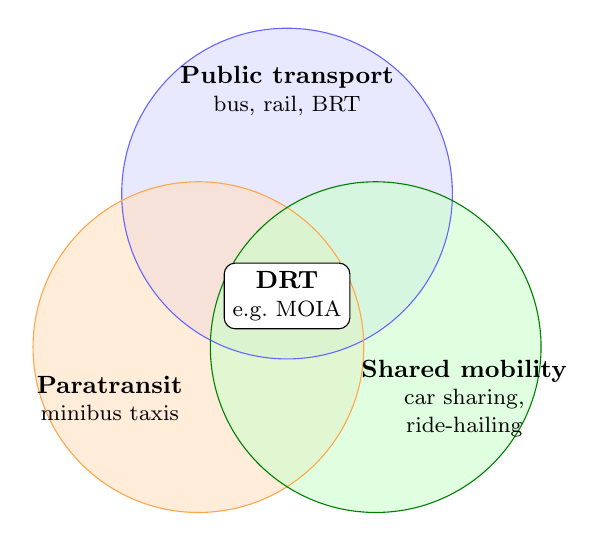
\begin{tikzpicture}[font=\small]
  \def\vennr{2.1cm}
  \fill[blue!15, opacity=0.6]   (90:1.3cm)  circle (\vennr);
  \fill[orange!25, opacity=0.6] (210:1.3cm) circle (\vennr);
  \fill[green!20, opacity=0.6]  (330:1.3cm) circle (\vennr);
  \draw[blue!60]   (90:1.3cm)  circle (\vennr);
  \draw[orange!70] (210:1.3cm) circle (\vennr);
  \draw[green!50!black] (330:1.3cm) circle (\vennr);
  \node[align=center] at (90:2.6cm)  {\textbf{Public transport}\\[-1pt]\footnotesize bus, rail, BRT};
  \node[align=center] at (210:2.6cm) {\textbf{Paratransit}\\[-1pt]\footnotesize minibus taxis};
  \node[align=center] at (330:2.6cm) {\textbf{Shared mobility}\\[-1pt]\footnotesize car sharing,\\[-1pt]\footnotesize ride-hailing};
  \node[draw, fill=white, rounded corners, align=center, inner sep=3pt] at (0,0) {\textbf{DRT}\\[-1pt]\footnotesize e.g.\ MOIA};
\end{tikzpicture}
\captionsetup{width=.9\textwidth}
\alex{replace figure}
\caption{TO BE REPLACED, PLACEHOLDER: Conceptual positioning of DRT at the intersection of public transport, paratransit, and shared mobility (based on \citealp{butler2020smart}).}
\label{fig:drt_classification}
\end{figure}

\absatz
The general need to improve transport in cities has been termed ‘smart urban mobility’\citep{butler2020smart} and is not limited to Cape Town.
A literature review on urban mobility scenarios by \citet{miskolczi2021urban} found that the most likely outcome is a slow shift to emerging technologies of ride sharing, electric and self-driving vehicles by 2030.
In this context, travel time is a key factor.
Travel time is essential in decisions to use transport modes such as DRT \citep{reck2020shared}, and high fares do not necessarily deter use of public transport \citep{tyrinopoulos2013factors}.
Thus, prioritising efficient transport for lower congestion and time costs is a good priority, and aligns well with the expectation of the literature of a shift to an increased use of DRT and similar emerging technologies.
\absatz
However, the real-world implications of a large-scale DRT service on transportation system determinants like congestion remain unclear.
\citet{butler2020smart} note the effects of DRT on congestion can be both positive and negative, because congestion is a complex phenomenon \citep{arnott1994economics}.
Congestion frustrates drivers with high fuel costs and travel times.
Those who use public transport often have long queues, overcrowding, and delays \citep{jennings2015finding}.
DRT can decrease cars per passenger and increase traffic flow because of adaptive planning, but pick up and drop-off zones may also increase congestion, and vehicle numbers can increase with higher accessibility or preference for low-occupancy vehicles.
These issues should be monitored in pilot studies after the simulation and tests are completed.
Furthermore, land use and urban planning must be designed to complement purely mobility-focused solutions to obtain the most efficiency \citep{jabbarpour2018applications}.
Small decreases in travel demand can have significant impacts on alleviating congestion and improving travel time \citep{vickrey1969congestion}.
This, however, requires particular conditions, as congestion often occurs not only because of physical bottlenecks \citep{arnott1994economics}.
\absatz
In that vein, a report by the International Network for Transport and Accessibility in Low Income Communities (INTALInC) highlights the need for comparative studies that match local contexts \citep{lucas2019transport}.
Simulations with locally calibrated data fill this gap and harness the power of big data to help understand and solve social problems.
This would also be in line with \citet{vanderschuren2018ride}, who evaluated the potential market for ridesharing in Cape Town using the 2013 national transport survey data.
Their research, however, is constrained by a lack of quantitative data and relies on expert opinion alone.
Using ABM to simulate the city transport system, however, addresses this challenge of limited data availability and opens up the possibility for an evaluation of experimental policies such as the introduction of large-scale DRT.
% and we can investigate the author's conclusions that low income households would switch to ridesharing solutions and DRT could have a vital role to play in this regard , hence serving transport demand in the city.
\absatz
A simulation of Hamburg, Germany's MOIA service, a ridepooling service for up to five passengers in fully electric autonomous vehicles and varying fleet sizes and service areas \citep{KagerbauerKostorzWilkes2021_1000141282} finds that increasing the use of DRT has a positive effect on the use of public transport rather than 'cannibalising'\hypertarget{todo:lit-cannib-framework}{}\alex{this is the first time cannibalization is mentioned, should we explain the theoretical t Framework of DRT-Transit Integration vs. Cannibalization?} it, which is often a hypothetical argument against introducing DRT.
Furthermore in their research the large fleets with autonomous vehicles lead to the lowest costs \citep{KagerbauerKostorzWilkes2021_1000141282}.
Others \citep{Basu.2018} find that ride-pooling services serve as a complement to public transport and increase the efficiency of the overall system by serving as a feeder to the transit system.
On the contrary, it has been highlighted that introducing on-demand services comes with the potential threat of public transport cannibalized by shared DRT \citep{Oh.2020}.
Simulations for Jerusalem \citep{BenDor.2022}, Berlin \citep{Kaddoura.2020}, and the Rouen Normandie metropolitan area \citep{Vosooghi.2019} also indicate that cannibalization of the existing public transport sector by DRT must be avoided.\hypertarget{todo:lit-cite-kaddoura}{}\alex{Check Kaddoura.2020 citation (verify whether it supports the PT cannibalization claim).}
Therefore, the introduction of 'push factors'—measures that make private car use less attractive (e.g., higher parking fees or congestion tolls)—might be necessary.
As presented in this literature overview, there are many studies on DRT simulations and outcomes, but none focus on congestion and in particular not in the context of the Global South. \hypertarget{todo:lit-yanetsi-table}{}\yanetsi{Add a small comparison table: study · city · model · congestion? · cannibalization? · Global South?}
This study attempts to fill this research gap.\hypertarget{todo:lit-gap-weak}{}\leif{Not clear/strong enough.}\hypertarget{todo:lit-sim-subsec}{}\leif{I think I see the reviewer's point. For a simulation paper, there is basically no critical reflection of simulation papers. I would add an entire subsection of simulation studies that debate the status quo in literature in agent-based modelling etc.}
\hypertarget{todo:lit-yanetsi-hyp}{}\yanetsi{State hypotheses for both congestion and cannibalization}
\hypertarget{todo:lit-yanetsi-theory}{}\yanetsi{One paragraph of theory: what cannibalization is, when it is likely (short trips, low DRT fares, poor PT), and the opposite effect (DRT as feeder)}
%A research theme losely related to DRT is Mobility-as-a-Service (MaaS). The idea behind MaaS is to have integrated transport offerings within city or regional systems \citealp{Loubser} Such motivation-based policies offer higher efficiency and lower emissions \citep{maggi2021price}. DRT is often seen as playing a key role in MaaS. Since the simulation in this work will primarily have time and price-based switching, it can be interpreted as a lower bound of modal switching without preference influencing policy or marketing being implemented to increase the switching.


%% ============================================================================
%% METHOD
%% ============================================================================
\hypertarget{todo:method-concepts}{}\hypertarget{todo:method-yanetsi-bias}{}\section*{Method}
\leif{According to the second reviewer comment, I would try to include a new section trying to explain the transport economics/science concepts, such as cannibalization etc.}
\yanetsi{Add a short bias table to the Method}
To analyze the effects of significant changes to mobility services, we compare the status quo with a hypothetical case that introduces a large fleet of shared demand-responsive vehicles that Cape Town's population may use.
Taking advantage of ABM simulations, we are able to deal well with complexity and individual decisions, which gives confidence in the predicted change in congestion we investigate \citep{ronald2015simulating}.
For this, we fall back to the open source framework MATSim that allows traffic system modeling via ABM.
The number of cities with MATsim modeling frameworks and applications has been increasing across the world and includes Bremerhaven, Berlin, S\~{a}o Paulo, Lille Metropolis, Santiago de Chile, Z\"{u}rich, Basel, Vienna, Lagos, Casablanca, Cape Town and the San Francisco bay area \citep{schluter2021impact, maciejewski2016congestion, Kaddoura.2020, sallard2020agent, kickhofer2016creating, balac2021synthetic, diallo2021agent, ilahi2019existing, kagho2019agent, becker2018matsim, muller2021matsim, benhlima2021towards}.
%Literature on DRT simulation has been investigated by \citealp{ronald2015simulating}, and they highlight ABM to be a valuable tool to simulate DRT before implementing the modeled intervention.
%ABM uses network theory and focuses on individuals in a system, which allows for interaction between operators and users. \\
%because its highly disaggregated level of analysis allows us to investigate the effects of transport policies on travel behavior in a granular way.
\absatz
The upcoming section presents a general overview of MATSim and parameters used in this paper, followed by a description of the Cape Town scenario setup and an overview of the shared mobility scenarios applied.

\hypertarget{todo:method-yanetsi-drt-mod}{}\subsection*{MATSim framework and scenario parameters}
\yanetsi{Explain more of how DRT is modelled?}
MATSim represents travellers in the real world as artificial agents with corresponding socio-demographic attributes and aims to mimic real-world travel patterns through an co-evolutionary algorithm \citep{nnene2023simulation}.
The framework simulates daily activity and mobility patterns of all agents and takes into account mode choice, departure time and route choice.
Movement patterns of road vehicles are simulated on a network graph, which represents local infrastructure and carries attributes such as maximum free speed or road capacity.
Interaction between agents on network links with full capacities leads to congestion, which is handled in a queue-based first-in-first-out (FIFO) principle \citep{Horni.2016}.
\absatz
An integral part of MATSim ability to reproduce real-world mobility patterns is the optimization of agents' behavior through a maximization of an individual utility score that takes into account the time spent at planned activities and the time and cost spent travelling from one destination to another.
In a MATSim simulation, each agent iteratively performs a plan that expresses its preferences in terms of activities, trips and scheduling.
Over the course of the iterations, a set of agents modify their plans while others stick to their initial plans.
To compare plans with each other, each plan is given a score according to a utility function as described below.
The simulation ends after a predefined number of iterations, at which point an equilibrium is reached where no agents can further improve their score.
\absatz
The utility function is formulated as follows:

\begin{equation}
S_{\text{plan}} = \sum_{q=0}^{N-1} S_{\text{activity},q} + \sum_{q=0}^{N-1} S_{\text{travel},\text{mode}(q)}
\label{1}
\end{equation}

with

\begin{equation}
\begin{aligned}
S_{\text{travel},\text{mode}(q)} =\ & C_{\text{mode}} + \beta_{\text{trav},\text{mode}(q)} \times t_{q} \\
& - \beta_{m} \times \left( \gamma_{d,\text{mode}(q)} \times d_{\text{travel},q} + DMC_{\text{mode}} \times \lambda_{\text{mode}} \right) \\
& + \beta_{\text{transfer},\text{mode}(q)} \times x_{\text{transfer},q}
\end{aligned}
\end{equation}

where $q$ refers to a leg as part of a trip from origin to destination, $C$ is a mode-specific utility constant, and $\beta_{\text{trav},\text{mode}}$ is the marginal utility of traveling per hour (where congestion extends travel time and thus negatively impacts utility).
$\beta_{m}$ denotes the marginal utility of money spent on the trip, which equals one throughout the scenario.
The term $\gamma_{d,\text{mode}(q)} \times d_{\text{travel},q}$ accounts for distance-based costs (in meters multiplied by a distance rate).
Additionally, a daily monetary cost $DMC_{\text{mode}} \times \lambda_{\text{mode}}$ is incurred.
Here, $\lambda_{\text{mode}}$ is a boolean variable that equals 1 if the agent uses a particular mode for the first time on a given day and 0 otherwise.
This fee can be interpreted as representing vehicle fixed costs or subscription fees for public transport or demand-responsive transport (DRT).
$\beta_{\text{transfer},\text{mode}} \times x_{\text{transfer},q}$ represents a transfer penalty applied when agents must switch vehicles within a trip leg (e.g., for public transport legs) \citep{Horni.2016}.
\absatz
Table~\ref{Utility values} lists the mode-specific utility values and pricing parameters used for Cape Town.
Mode-dependent utilities for agents in Cape Town were established by adjusting values of the well-established Berlin scenario \citep{Ziemke.2019} until mode share and congestion calibration targets of Cape Town were met to match local sociodemographic characteristics and travel dynamics (for further information on the calibration exercise, see section below).

\begin{table}[H]
\centering
\caption{Varying utility and pricing parameters for different transportation modes available in the simulation.}
\label{Utility values}
\small
\begin{tabularx}{\textwidth}{l *{5}{>{\centering\arraybackslash}X}}
\toprule
\textbf{Mode} & \textbf{Constant} ($C$) & \textbf{Daily monetary constant} ($DMC$) & \textbf{Marginal utility of travelling} ($\beta_{\text{trav}}$) & \textbf{Monetary distance rate} [ct/km] ($\gamma_{d}$) & \textbf{Transfer utility} ($\beta_{\text{transfer}}$) \\
\midrule
Public transport & 0 & $-1.9$ & 0 & 0 & $-1$ \\
Car              & 0 & $-10$  & 0 & $-11$ & 0 \\
DRT              & 0 & varying & 0 & varying & 0 \\
\bottomrule
\end{tabularx}

\end{table}

It becomes evident that, under this modeling setup, travel time using a particular mode does not directly impact an agent's (dis)utility while traveling.
However, longer travel times reduce the time available for activities (captured by the first term in equation~\ref{1}), indirectly lowering the agent’s overall score.
Consequently, agents will seek to avoid traffic congestion, as increased travel time decreases their utility.
We explicitly acknowledge, however, that Cape Town travellers may exhibit additional behavioural inertia (e.g., distrust in shared or public rides or preference for private-car autonomy even under congestion) that is not fully captured by the utility function.
The simulation outcomes should therefore be interpreted as the potential congestion relief if mode choice behaviour aligns with the modelled rational response.
\hypertarget{todo:method-intermodal}{}\alex{Reviewer critic Cannibalization modelling: Make it clear that agents can or cannot perform intermodal mobility trips (i.e. different mode legs during a trip) }

\hypertarget{todo:method-drt-mech}{}\alex{new subsection? Explain MATSIM-internal DRT mechanism}
\hypertarget{todo:method-yanetsi-cannib}{}\yanetsi{Cannibalization: Say which model parts capture it: mode choice, prices in Eq. 2, PT times from GTFS, whether DRT+PT trips are possible}


\hypertarget{todo:method-rev4-data}{}\hypertarget{todo:method-yanetsi-years}{}\subsection*{Baseline Cape Town MATSim scenario and calibration}
\timo{Reviewer Comment 4 (Reduce Study Biases): Use more current / overlapping data. Try to ``update'' the whole study.}
\yanetsi{Data from 2011, 2013, 2018, 2022: list the years and discuss}

A synthetic scenario of Cape Town with a population sample size of 10\,\% is employed for the study.
We derive the synthetic population from South African Census Data 2011 \citep{census2011}, the 10\,\% Public Use Sample \citep{census2011public10pct} and the Minnesota Population Center Integrated Public Use Microdata Series \citep{mpc2020}.
For the population synthesis process we employ a multi-level iterative proportional fitting methodology.
Furthermore, we utilize data from National Household Travel Survey 2013 \citep{nhts2013} and the Time Use Survey 2010 \citep{tus20NationalHouseholdTravelSurvey13} to assign individual mobility behaviour to the synthetic agents.
\absatz
On the supply side we employ network and infrastructure data from OpenStreetMap (OSM) \citep{osm}.
The network links are downscaled according to the population sample in terms of flow and storage capacities.
Furthermore, the individual OSM IDs of the dataset are extracted and categorised into different activities such as "shopping" or "leisure".
In addition, we use GTFS datasets from the main public transport providers in Cape Town from 2018 to model public transport \citep{transifeeds}.
The capacities of the public transportation vehicles are also downscaled according to the population sample (1:10), as the adjustment of the vehicle size to the downscaled network leads to a distortion of the passenger flows.
To avoid further distortions in the timetables of the vehicles by the other network participants and for reasons of simplification, the vehicles of Golden Arrow Bus Services (GABS), Metrorail Western Cape, MyCiTi Cape Town Integrated Rapid Transit (IRT) system and the University of Cape Town's (UCT) campus shuttle buses operate on a pseudo-network with direct aerial lines between stops and with adjusted speed limits on each route to match the timetable.
For the modelling of informal public transport in the form of minibus taxis, the use of a pseudo-network is omitted due to the fact that the number of minibus taxis is significantly higher than in the case of formal public transport which leads to feedback effects in the traffic flow.
To represent these effects in the overall traffic in Cape Town the Minibus Taxis travel together with the other individual traffic on the OSM motor roads.
\absatz
Again, using the OSM data, the modelled infrastructure and the socio-demographic characteristics of the agents such as age, gender and employment status, a gravity model is used to create a path-destination matrix and assign it to the agents.
The resulting base population then goes through several calibration steps to accurately mimic the real world travel patterns, calibrating towards NHTS averages and Cape Town Vehicle Detection System (VDS) traffic flow data on major roads from 2018.
The calibration target is set at an average deviation from real data of less than 20\,\% error for car traffic and less than 50\,\% for formal and informal public transport.
\absatz
Figure \ref{fig:x_1} shows the location of traffic count station the simulation was calibrated against.
Moreover, it depicts the average free flow speed divergences in km/h on major streets during a weekday rush hour between 4 and 5 pm based on TomTom traffic analysis data from October 2022.
Figure \ref{fig:x_2} shows calibration results of an example count station.
This goes to show that the model is fit well against major mobility patterns, in particular traffic delays.

\begin{figure}[H]
\centering
\hypertarget{todo:fig1-timo}{}\hypertarget{todo:fig1-leif}{}\hypertarget{todo:method-yanetsi-tomtom}{}%
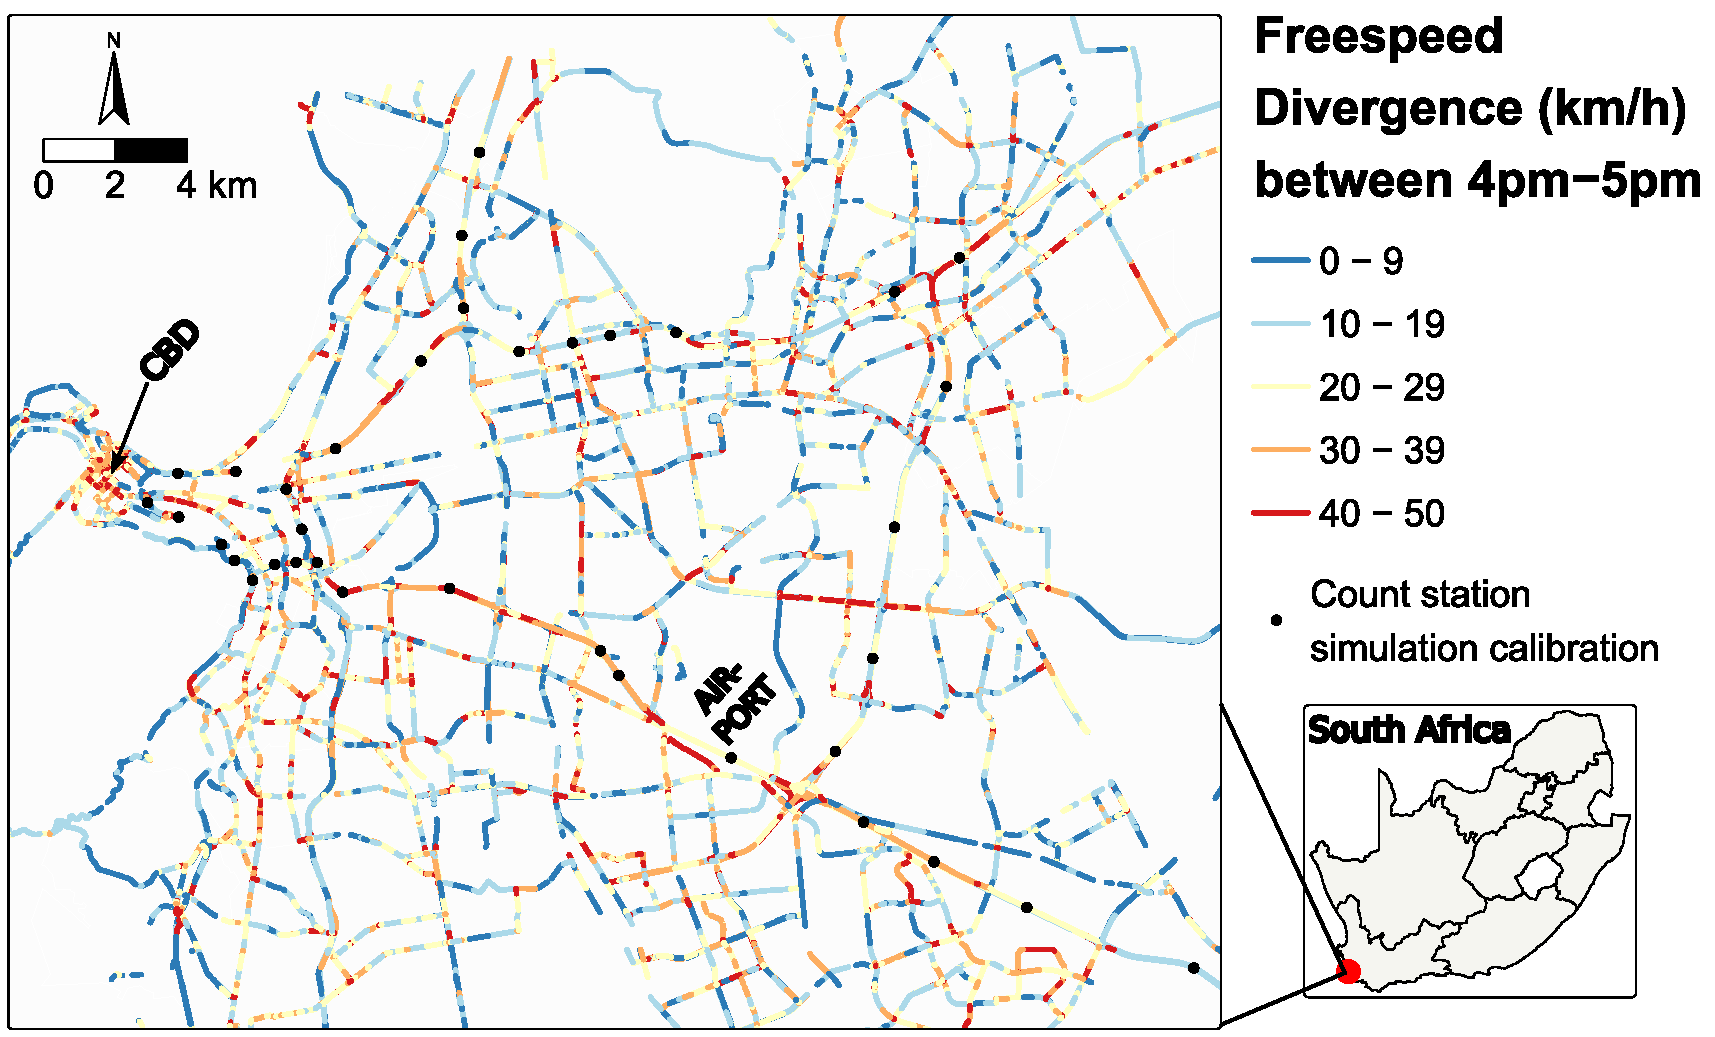
\includegraphics[width=1\textwidth]{images/Meine_Karte_mit_Inset_22_cropped.pdf}
  \captionsetup{width=.8\textwidth}
  \caption{Free-flow speed divergence on major roads in Cape Town on an average Wednesday in October 2022 (Data: TomTom). Points depict traffic count stations that have been used to calibrate the simulation.}
  \label{fig:x_1}
  \timo{Fig. 1: Elaborate a bit more. What do we actually see? The CBD (Central Business District) is not explained.}
  \leif{Fig. 1: Since the points are the more significant point of including this figure, they should be more visible.}
\end{figure}

\yanetsi{TomTom data over-represents drivers with navigation apps: discuss, compare with travel-survey flows}
For our chosen measure of traffic congestion, the difference between the free flow speed and the actual simulation flow speed is aggregated for each street link on a daily basis. \hypertarget{todo:method-alt-cong}{}\alex{look for alternative measurements of congestion?}
As noted earlier, since scheduled transport operates on artificial links that have no intersections with links corresponding to the real world, we account only for congestion caused by cars and minibus taxis, which make up the vast majority of traffic on Cape Town's streets.

\begin{figure}[H]
\centering
\hypertarget{todo:fig2-timo}{}\hypertarget{todo:fig2-leif}{}%
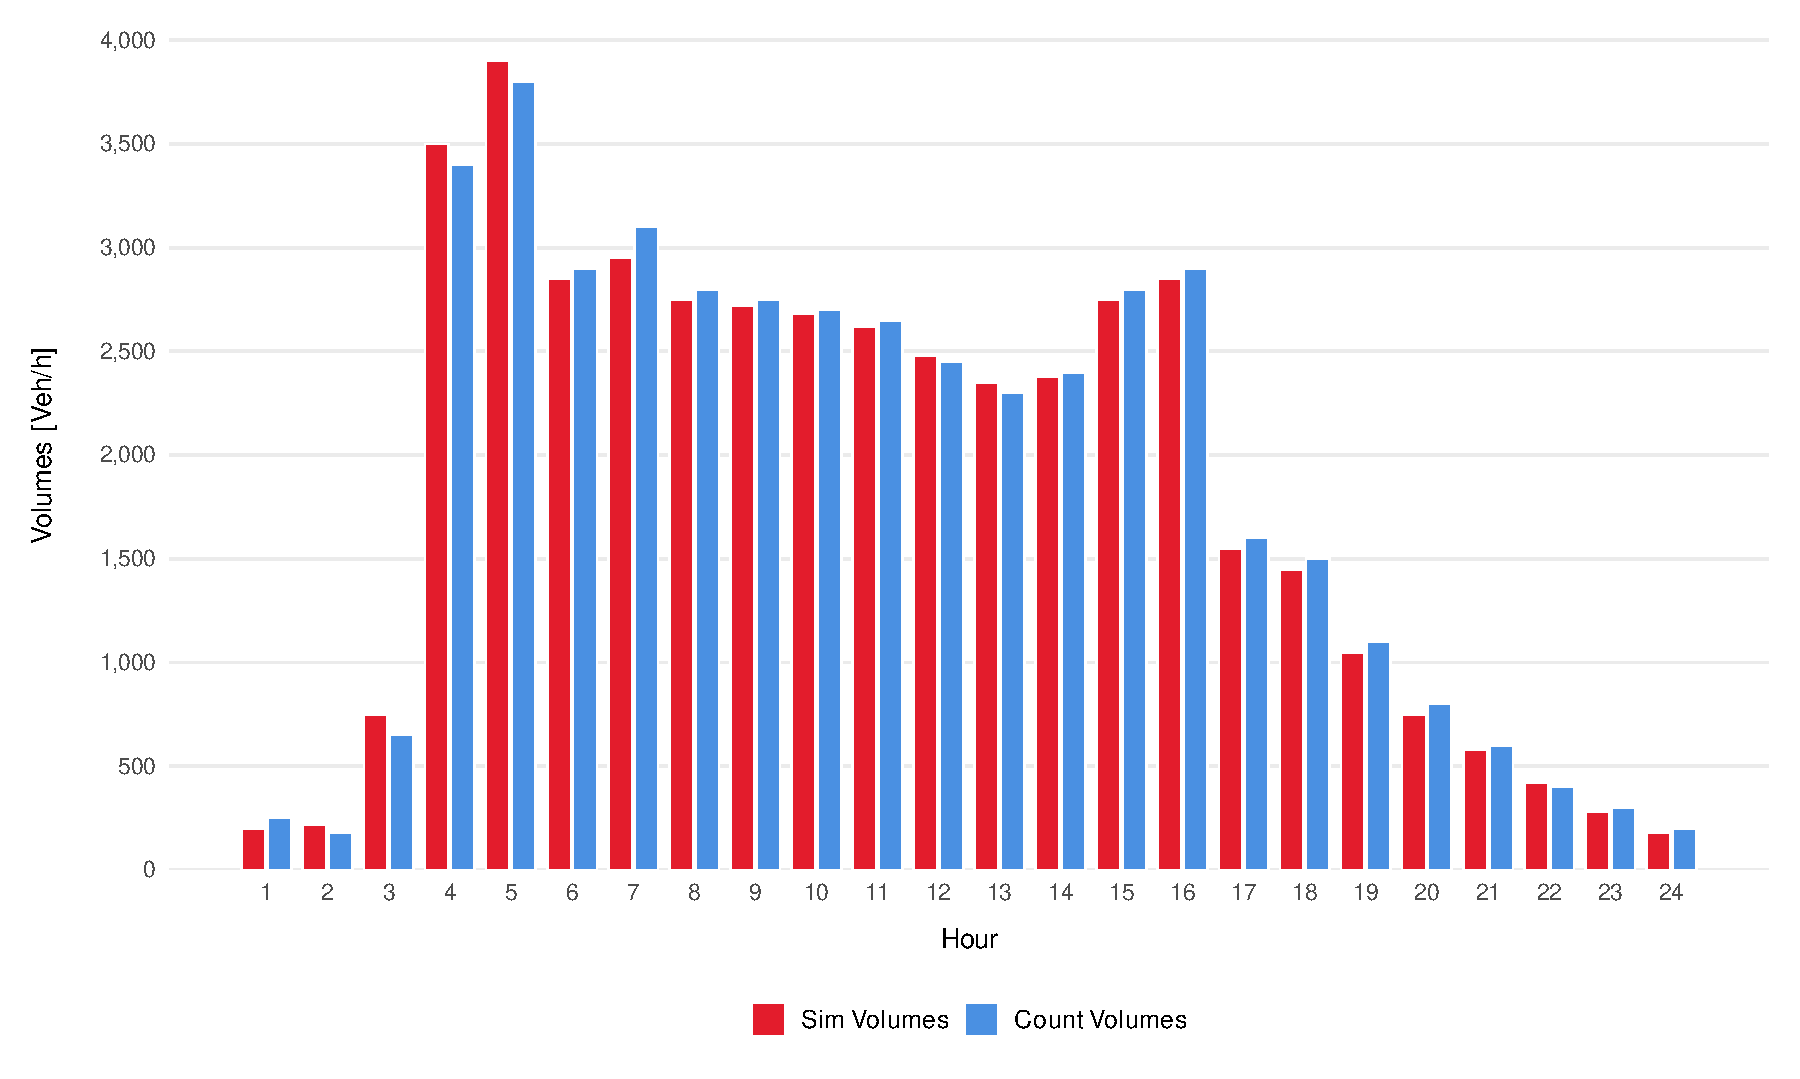
\includegraphics[width=1\textwidth]{images/airport_count_station.pdf}
  \captionsetup{width=.8\textwidth}
  \caption{Simulation calibration results for traffic count station near airport.}
  \label{fig:x_2}
  \timo{Fig. 2: Recreate the figure using the mean of all counting stations, and include standard deviation as error bars for each hourly bar.}
  \leif{Fig. 2: More info on this figure. Are those averages? Is it weekdays? Can we come up with a figure of ``accuracy'' instead of just showing a bar plot?}
\end{figure}

\begin{figure}[H]
\centering
\definecolor{simred}{RGB}{220,34,42}
\definecolor{countblue}{RGB}{72,136,228}
\begin{tikzpicture}
\begin{axis}[
    ybar=1.5pt,
    bar width=4.2pt,
    width=\textwidth,
    height=7.5cm,
    ymin=0, ymax=4400,
    ytick={0,500,1000,1500,2000,2500,3000,3500,4000},
    ymajorgrids=true,
    grid style={gray!28},
    axis x line*=bottom,
    axis y line*=left,
    y axis line style={draw=none},
    ytick style={draw=none},
    xtick style={draw=none},
    xtick={1,2,...,24},
    enlarge x limits=0.03,
    xlabel={Hour},
    ylabel={Volumes [Veh/h]},
    tick label style={font=\scriptsize},
    label style={font=\small},
    legend style={
        at={(0.5,-0.16)},
        anchor=north,
        legend columns=2,
        draw=none,
        font=\small,
        /tikz/every even column/.append style={column sep=12pt}
    },
    legend image code/.code={
        \draw[#1, draw=none] (0cm,-0.1cm) rectangle (0.28cm,0.18cm);
    },
    error bars/y dir=both,
    error bars/y explicit,
    error bars/error bar style={black!75, line width=0.5pt},
    error bars/error mark options={rotate=90, mark size=1.4pt, line width=0.5pt, black!75}
]
\addplot[fill=simred, draw=none] coordinates {
    (1,195)+-(0,35)   (2,215)+-(0,38)   (3,740)+-(0,110)  (4,3480)+-(0,340)
    (5,3890)+-(0,380) (6,2840)+-(0,290) (7,2950)+-(0,310) (8,2740)+-(0,280)
    (9,2710)+-(0,270) (10,2675)+-(0,260)(11,2610)+-(0,255)(12,2480)+-(0,245)
    (13,2340)+-(0,235)(14,2375)+-(0,240)(15,2745)+-(0,275)(16,2840)+-(0,285)
    (17,1545)+-(0,180)(18,1445)+-(0,170)(19,1045)+-(0,130)(20,745)+-(0,100)
    (21,575)+-(0,85)  (22,415)+-(0,65)  (23,275)+-(0,48)  (24,175)+-(0,32)
};
\addplot[fill=countblue, draw=none] coordinates {
    (1,245)+-(0,42)   (2,180)+-(0,35)   (3,645)+-(0,105)  (4,3390)+-(0,355)
    (5,3795)+-(0,395) (6,2890)+-(0,305) (7,3095)+-(0,325) (8,2795)+-(0,295)
    (9,2745)+-(0,285) (10,2700)+-(0,275)(11,2645)+-(0,270)(12,2445)+-(0,255)
    (13,2290)+-(0,245)(14,2395)+-(0,250)(15,2795)+-(0,285)(16,2895)+-(0,295)
    (17,1595)+-(0,190)(18,1495)+-(0,180)(19,1095)+-(0,140)(20,795)+-(0,110)
    (21,595)+-(0,90)  (22,395)+-(0,65)  (23,295)+-(0,52)  (24,195)+-(0,38)
};
\legend{Sim Volumes, Count Volumes}
\end{axis}
\end{tikzpicture}
\captionsetup{width=.85\textwidth}
\caption{PLACEHOLDER / SAMPLE DATA: Mean hourly simulated and observed traffic volumes across all counting stations with 95\,\% confidence intervals (illustrative sample plot matching the visual style of Figure~\ref{fig:x_2}; replace with empirical multi-station statistics).}
\label{fig:x_2_sample_ci}
\end{figure}

\hypertarget{todo:method-yanetsi-drt-params}{}\hypertarget{todo:method-yanetsi-eligibility}{}\hypertarget{todo:method-yanetsi-booking}{}\subsection*{DRT scenarios and parameterization}
\yanetsi{vehicle capacity, max waiting time, max travel time α/β, operating hours; rest at defaults?}
\yanetsi{Limit who can book DRT (e.g. income, age, smartphone ownership) and state the rule}
\yanetsi{One paragraph on booking and information: what the model assumes (perfect information, instant booking) and what it ignores (digital access, trust, safety)}

The main objective of this study is to analyze whether introduction of a large-scale DRT fleet is able to reduce congestion by encouraging a modal shift from private cars to DRT while prevent public transport cannibalization by the new introduced mode.
To achieve this, we design a service area where agents who begin or end their trips within the designated area have the option to switch to DRT.\hypertarget{todo:method-yanetsi-counterfactual}{}\yanetsi{Introduce counterfactual service areas to prevent fishing-for-results-bias}
Other service type options like the introduction of a stop-based DRT system are not considered because they would resemble the existing paratransit systems to a large extent.
In our service-area based approach, agents can ride-hail DRT vehicles when the start and end of their trip falls within the defined service area.
\absatz
We design the DRT service area using a two-step process. \hypertarget{todo:method-yanetsi-buffer}{}\yanetsi{state 1000m buffer zone}
First, we identify wards with the highest car trip activity.
Second, we combine these with wards that have a high concentration of upper-middle-income households to create a final service area that captures a large share of car trips while targeting users who are more likely to afford and use the service.
\absatz
Using origin-destination car trip data from TomTom (2022), we calculate the share of inter-ward car trips for every origin-destination ward pair in Cape Town.
We rank these ward pairs in descending order based on their contribution to total car trips and compute the cumulative share.
By applying a 60\,\% coverage threshold, we select all wards that appear in at least one of the top-ranked origin-destination pairs.
Figure~\ref{fig:x_5} shows the spatial distribution of car trip origins.
Car usage remains particularly high in the more affluent suburbs surrounding the city's major economic hubs (CBD, Kenilworth, and Bellville).

\begin{figure}[!h]
\centering
\hypertarget{todo:fig3-timo}{}%
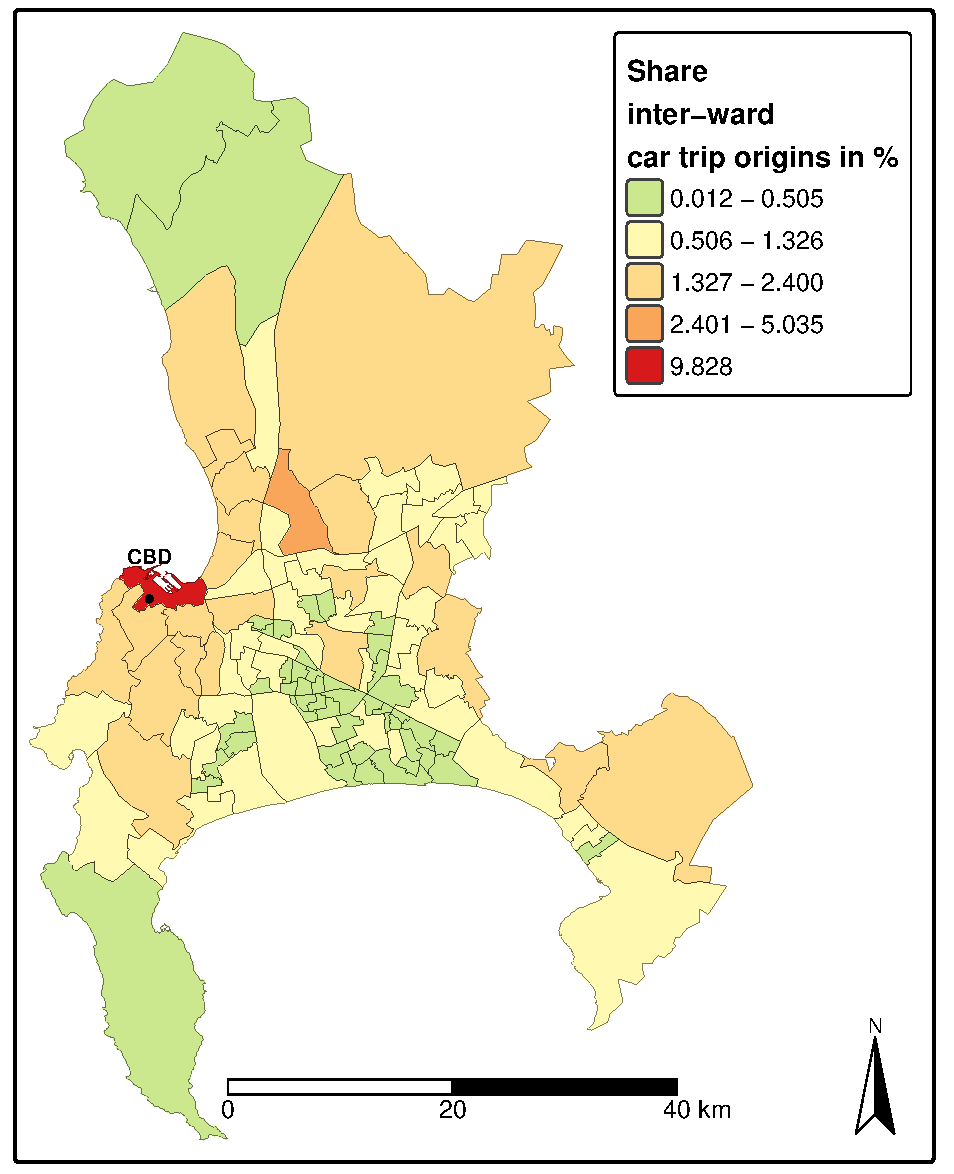
\includegraphics[width=0.6\textwidth]{images/inter-wards_car_trips_origins_edit-3_cropped.pdf}
\captionsetup{width=.9\textwidth}
\caption{Share of inter-ward car trip origins per ward in \% (Data: TomTom 2022).}
\label{fig:x_5}
\timo{Fig. 3: Address why outer regions are unattractive for DRT (due to distance / pricing?). Also, mark the airport clearly.}
\end{figure}

DRT functions as a hybrid between public transportation and private car use.
Therefore, its fares are expected to be higher than conventional public transport but lower than the full cost of driving a private car.
We target neighborhoods with a high concentration of upper-middle-income households that have greater financial capacity to pay for a higher-quality on-demand service.
Additionally, market-based solutions like DRT could help alleviate the lack of public infrastructure \citep{TDCIP}.
Using data from the 2011 South African Census \citep{census2011}, we identify wards with the highest share of upper-middle-income households (annual household income between ZAR\,76,801 and ZAR\,614,400, \$13,798.24 – \$110,384.5 PPP).
These wards are then combined with the high car-usage wards from Step 1 to define the final DRT service area.
\absatz
This service area, marked by the blue boundary in Figure~\ref{fig:x_3}, covers 83.7\,\% of all origin-destination car trips recorded by TomTom, making it a well-targeted region with high car traffic, congestion, and private car usage, particularly in key business centers across the city.
The same figure also shows the baseline (no-DRT) traffic congestion levels in the study area.
In the baseline scenario, congestion causes approximately 253,000 hours of additional travel time, accounting for 86\,\% of total car travel time in the region.
Congestion inside the designated DRT service area (131,500 hours) is slightly higher than outside it (121,500 hours).

%\begin{figure}[!h] \centering 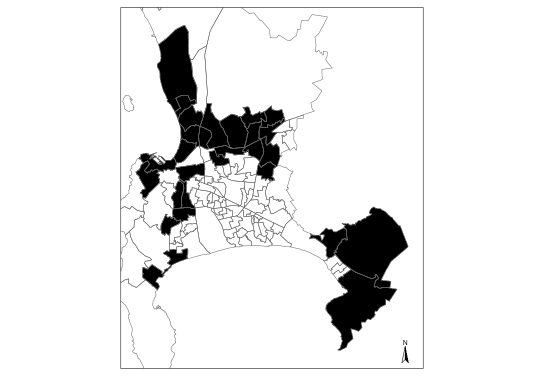
\includegraphics[width=1\textwidth]{images/service_area.png} \captionsetup{width=.9\textwidth} \caption{DRT Service Area} \label{fig:x_6} \end{figure}

\begin{figure}[H]
\centering
\hypertarget{todo:fig4-timo}{}%
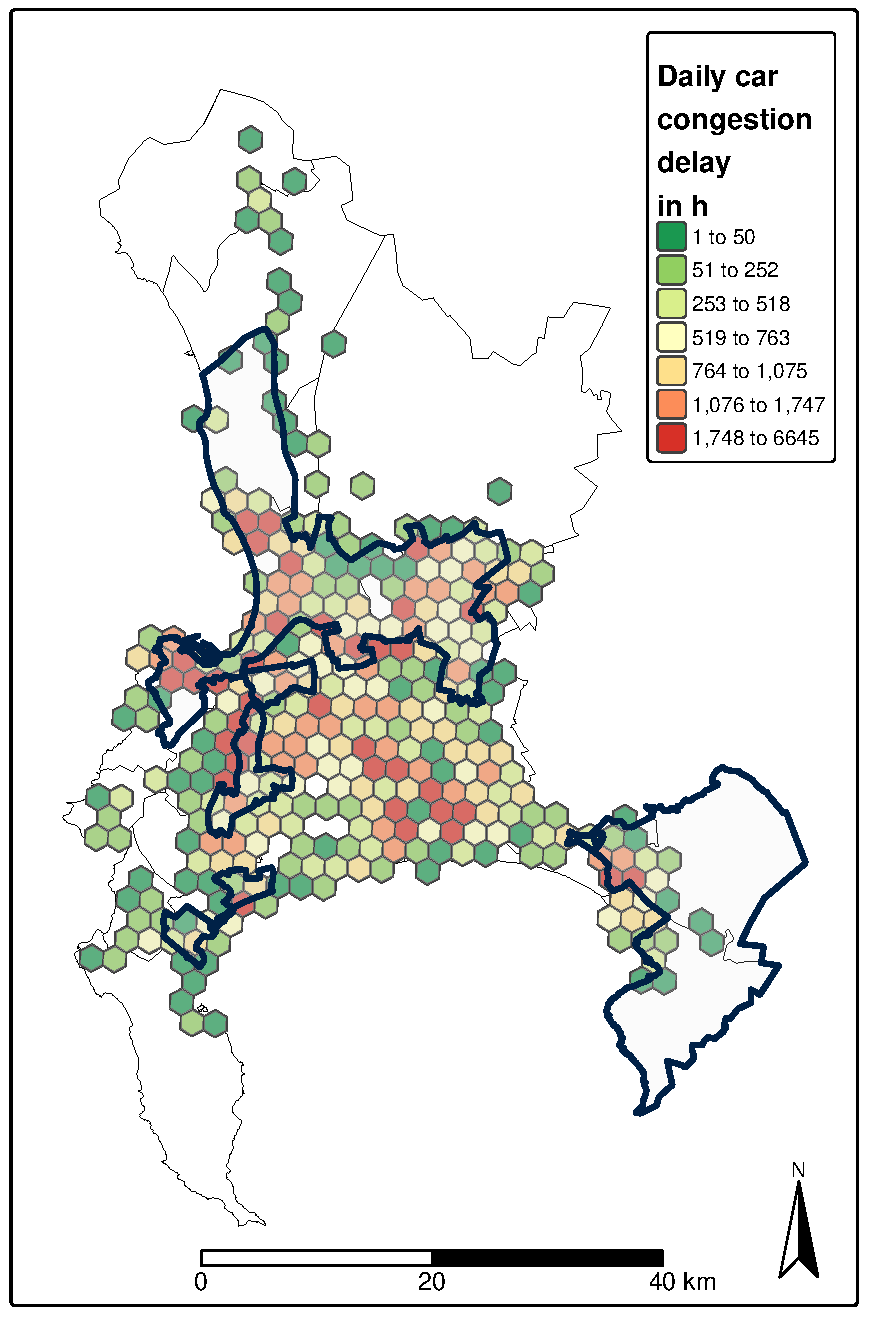
\includegraphics[width=0.6\textwidth]{images/daily_delay_basecase_edit-3_cropped.pdf}
\captionsetup{width=.9\textwidth}
\caption{Simulation baseline scenario: Spatial distribution of daily congestion. The blue-highlighted area marks the DRT service area constructed.}
\label{fig:x_3}
\timo{Fig. 4: Clarify if this represents congestion delay per person or per ride. Note heavy congestion around the airport (?), but check why there are not as many car trip origins compared to Fig. 3.}
\end{figure}

%\begin{figure}[H] \centering 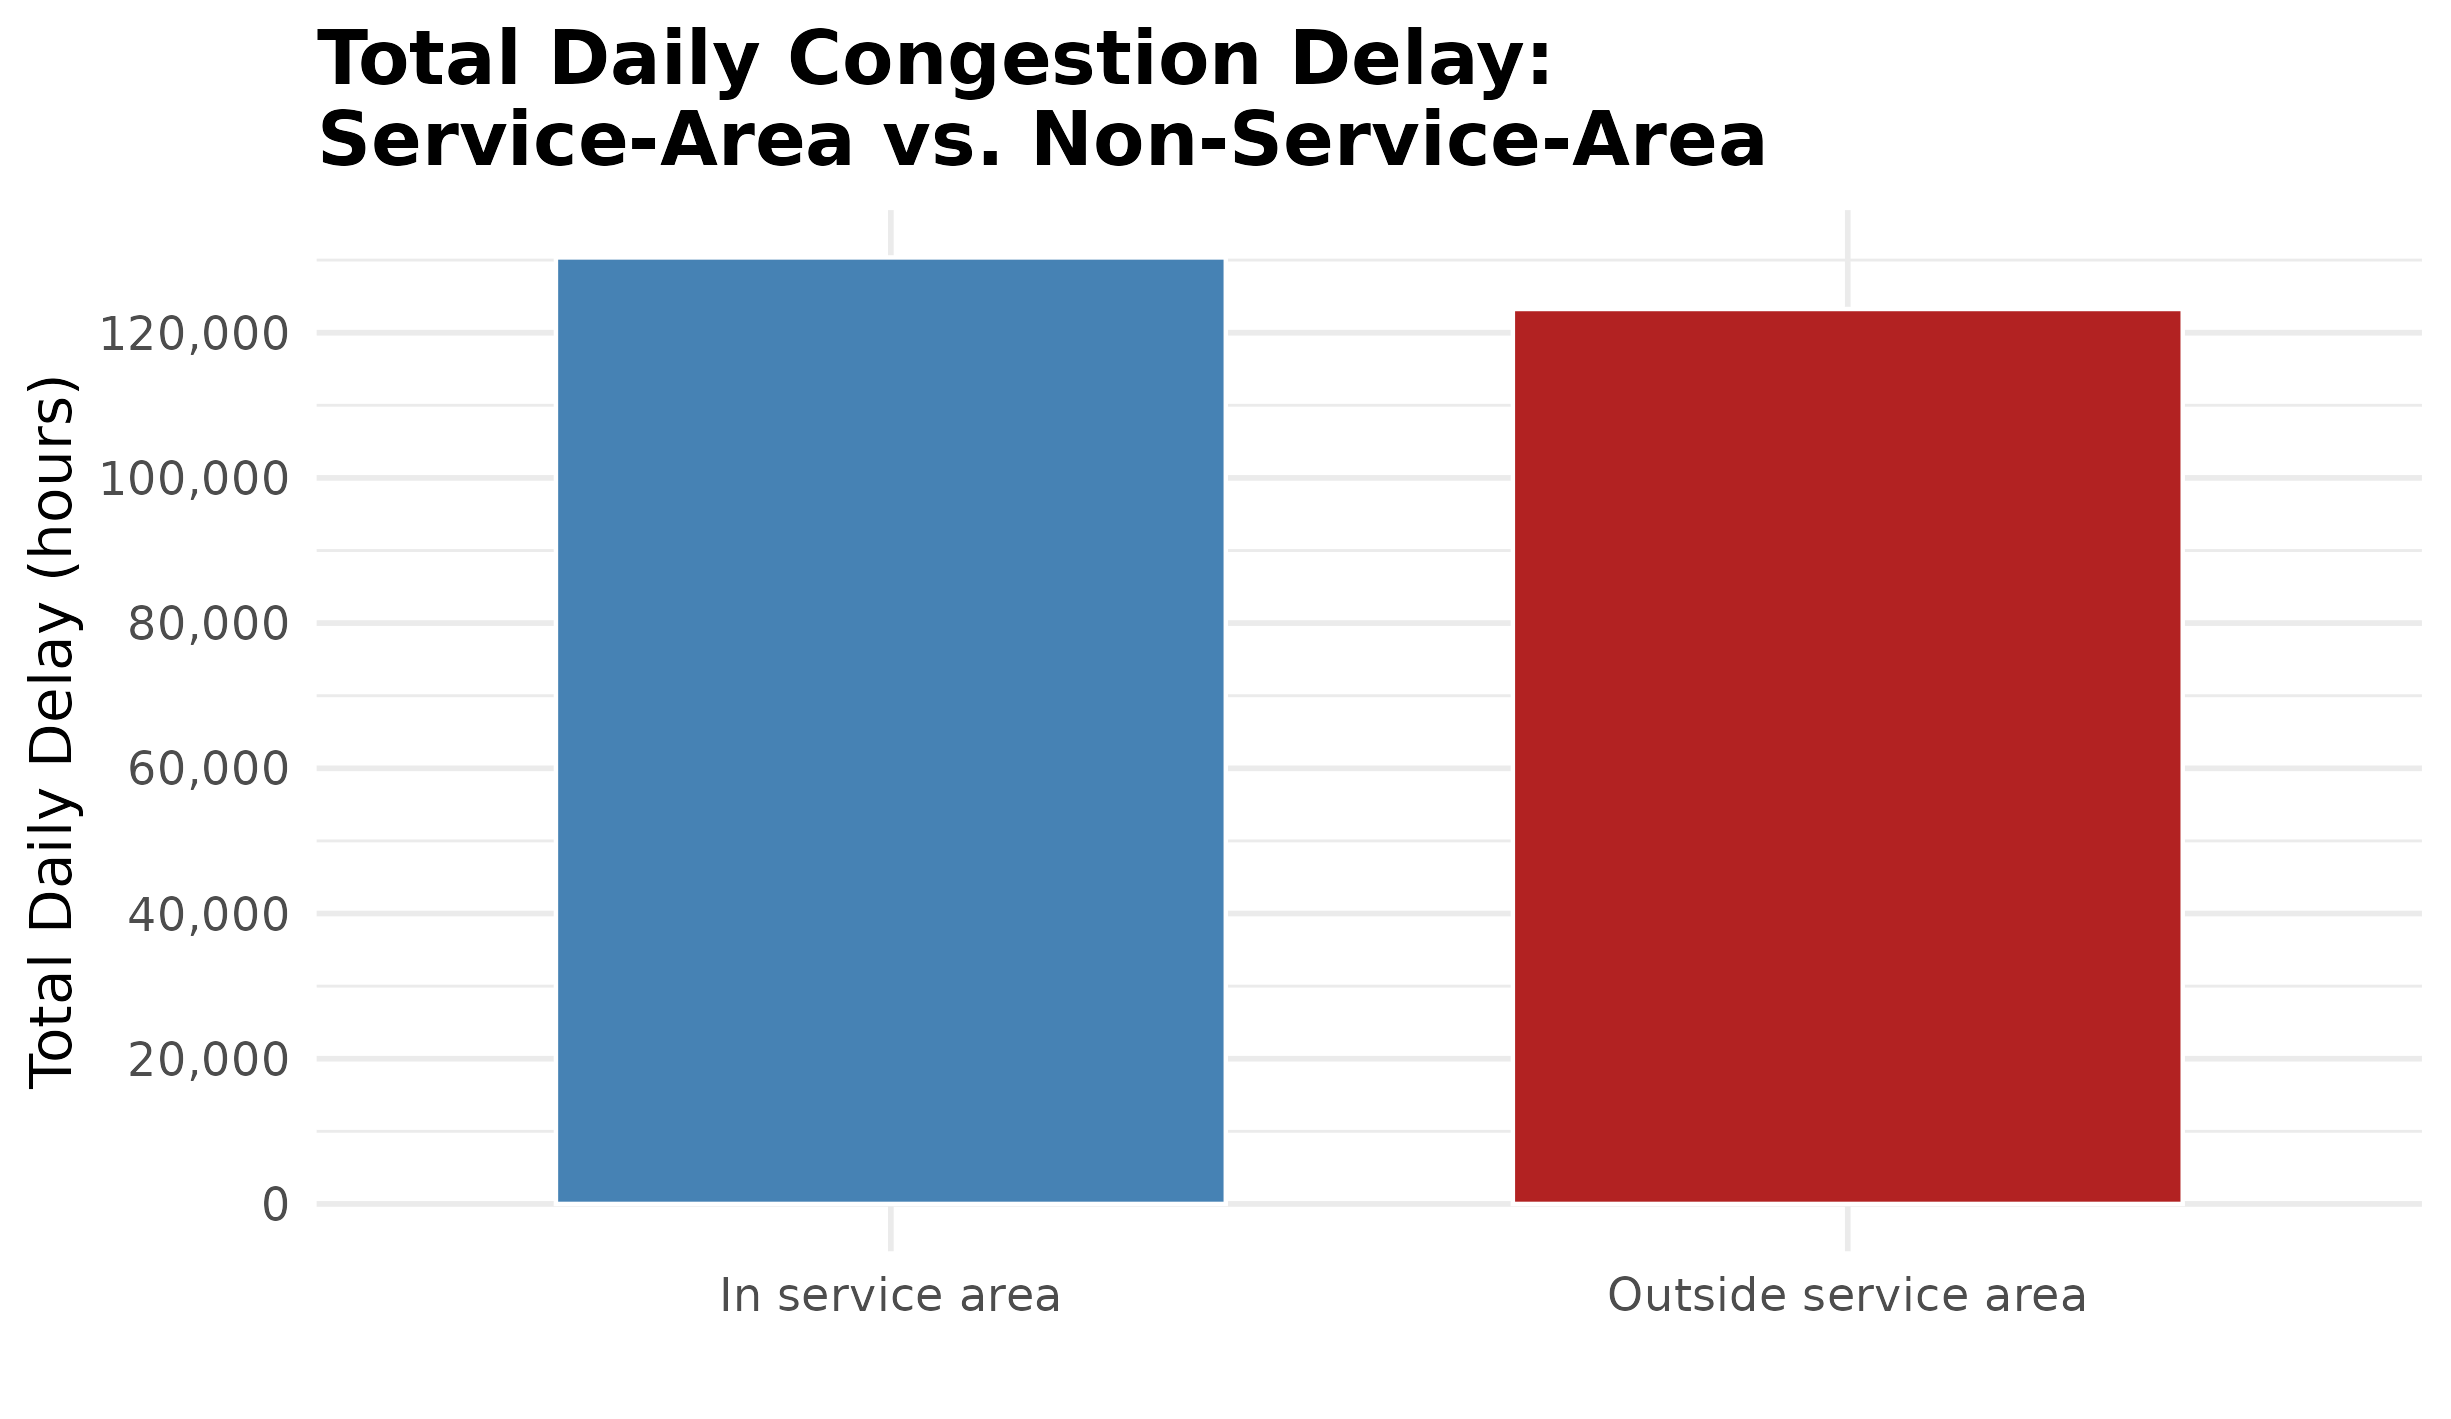
\includegraphics[width=0.8\textwidth]{images/baseline_total_congestion_service_area.png} \captionsetup{width=.9\textwidth} \caption{Simulation baseline scenario: Aggregate daily congestion in and outside of DRT service area} \label{fig:x_4}  \end{figure}

Several scenarios using different fleet sizes and pricing schemes are simulated to evaluate the potential impact on congestion.
The fleet sizes are based on a sample of total car drivers in the baseline MATSim scenario (52,775 drivers, or a 10\,\% sample).
We test fleet sizes equivalent to 0.5\,\%, 1\,\%, 1.5\,\%, and 2\,\% of the total car drivers in Cape Town (264, 528, 792, and 1056 vehicles, respectively).
\absatz
The pricing factor plays an essential role in shaping the choice of service areas.
Since higher-income areas are more likely to afford transport options that are priced higher than public transport, while lower-income areas already spend significant portions of their income on public transport, the pricing is adjusted to reflect these differences.
For the DRT pricing schemes, we vary both the mandatory one-time daily fee and the variable price per kilometer.
The daily fee is set to 200\,\%, 250\,\%, and 300\,\% of the daily fixed fee for public transport, while the variable distance price takes up the values from 45.45\,\%, 55.55\,\%, 65.65\,\%, 75\,\% and 100\,\% of the car km fee used in the baseline scenario.
Notably, the pricing structure of the DRT services deviates from ride-hailing services like Uber or Bolt in that the variable cost for shared DRT rides are split between the two or more passengers, making the trip cheaper than ride-hailing services on the same route.
Table \ref{tab:drt_parameters} presents all parameter dimensions and relevant values.
In total, we evaluate 60 different scenarios based on all value combinations of the parameter dimensions.

\begin{table}[h]
\centering
\hypertarget{todo:method-yanetsi-median-fee}{}%
\caption{Complete parameter grid for all 60 simulated DRT scenarios.}
\label{tab:drt_parameters}
\begin{tabularx}{\textwidth}{>{\centering\arraybackslash}X >{\centering\arraybackslash}X >{\centering\arraybackslash}X}
\toprule
\textbf{Fleet size (\% of daily car drivers)} & \textbf{Daily DRT fee (\% of PT daily fee)} & \textbf{Variable DRT fee (\% of car km fee)} \\
\midrule
0.5\,\%, 1.0\,\%, 1.5\,\%, 2.0\,\% & 200\,\%, 250\,\%, 300\,\% & 45.45\,\%, 55.55\,\%, 65.65\,\%, 75\,\%, 100\,\% \\
\bottomrule
\end{tabularx}
\yanetsi{Check the median scenario's km fee: 59.1\% is not in the Table 2 grid}
\end{table}

The pricing assumptions were selected to reflect realistic affordability thresholds for upper-middle-income households in Cape Town, who are more likely to adopt DRT as a viable alternative to private cars or existing ride-hailing services.
The daily fee levels were chosen as they represent a midpoint between low-cost public transport and higher car ownership costs (the latter being more than five times as high than the former), allowing us to observe the intended mode-shifting effects without making DRT prohibitively expensive.
For instance, a 200\,\% daily fee aligns with real-world pricing in similar contexts, such as Hamburg's MOIA service, where fares are approximately 2–3 times public transport rates to encourage uptake among affluent users \citep{KagerbauerKostorzWilkes2021_1000141282}.
The variable distance rates (45.45\,\% to 100\,\% of car km fees) enable further sensitivity analysis, specifically designed to test DRT's competitiveness below the full variable costs of cars.
By setting rates as low as 45.45\,\% (e.g., equivalent to a subsidized or efficiency-optimized fare), we capture scenarios where DRT incentivizes shifts from private cars—whose variable costs include fuel and maintenance—while remaining attractive relative to ride-hailing services like Uber or Bolt, which often charge 80–120\,\% of car km equivalents due to unshared rides and surge pricing \citep{Tirachini2020-sr}.
Higher rates (up to 100\,\% of the variable car price) simulate less subsidized operations, revealing potential thresholds where adoption drops and congestion relief diminishes. \hypertarget{todo:method-yanetsi-dispatch}{}\yanetsi{How does the DRT dispatching inside Matsim work?} \hypertarget{todo:method-yanetsi-wait}{}\yanetsi{Explain the concept of waiting time and potential pre-booking in the simulation}


%% ============================================================================
%% WORKING TABLE (YANETSI): EXPLANATIONS THAT CONTRADICT THE MODEL
%% ============================================================================
\ifshowtodooverview
\begin{table}[H]
\centering
\caption{WORKING TABLE (Yanetsi): Explanations in the Results/Discussion that contradict the MATSim model mechanics (hidden when \texttt{\textbackslash showtodooverviewfalse}).}
\label{tab:yanetsi_model_contradictions}
\footnotesize
\begin{tabularx}{\textwidth}{>{\raggedright\arraybackslash}X >{\raggedright\arraybackslash}X >{\raggedright\arraybackslash}X l}
\toprule
\textbf{Paper's explanation} & \textbf{Why the model can't produce it} & \textbf{Fix} & \textbf{Work} \\
\midrule
Road congestion speeds up or delays buses (Fig.~11) & Buses and trains run on a separate pseudo-network & Explain via minibus taxis, crowding, mix of trips & Writing \\
\addlinespace
Less stop-and-go, better routes & Queue model has no stop-and-go; DRT routes like cars & Queues are nonlinear: small cut in cars, large cut in delay & Writing \\
\addlinespace
Congestion rises at high prices because DRT is underused & Non-use gives baseline traffic, not more & Empty DRT vehicles + PT $\rightarrow$ car switches & Output \\
\addlinespace
More km but less congestion due to occupancy & Queues count vehicles, not passengers & Extra km driven off-peak or on roads with spare capacity & Output \\
\bottomrule
\end{tabularx}
\aitodo{Elaborate more on these points and explain the meaning behind all these points}
\end{table}
\fi

%% ============================================================================
%% RESULTS
%% ============================================================================
\hypertarget{todo:res-yanetsi-drt-cong}{}\hypertarget{todo:res-yanetsi-cannib-def}{}\section*{Results}
\yanetsi{Say whether DRT vehicles count in the congestion measure}
\yanetsi{Define cannibalization measures (DRT riders who came from PT; net change in PT trips and km) and report them for every scenario}
The introduction of DRT across 60 scenarios consistently reduced aggregate daily congestion compared to the baseline scenario, where additional travel time incurred from delays constitutes the majority of total travel time.
This aligns with findings by \citet{schluter2021impact}, who demonstrated significant reductions in congestion on rural-urban corridors through DRT implementations.
Figure \ref{fig:x_6} illustrates the impact of DRT introduction on car use (measured by total cars on the road) and total congestion.
The extent of reduction varied with DRT configuration, with scenarios featuring larger fleets and lower pricing achieving the greatest reductions, up to 28.2\,\% citywide.
In the median scenario, congestion decreased by 12.7\,\%, while the least effective scenarios (e.g., smallest fleet sizes at highest prices) still yielded a modest 2.5\,\% reduction.
This variability underscores that fleet size and pricing are critical levers for optimizing congestion relief potential of DRT, a point echoed by \citet{engelhardt2019quantifying} in their study on fleet optimization for shared mobility.
Notably, even in less effective configurations, DRT contributed to decongestion, highlighting its robustness as a mitigation strategy.
Scenarios with higher costs showed minimal shifts from car use, resulting in smaller congestion reductions, indicating that DRT's effectiveness hinges on its ability to compete with private cars on cost.
Moreover, it is notable that the relative decrease in congestion often exceeds the reduction in the total number of cars on the street.
This suggests that DRT not only reduces the number of vehicles but also enhances traffic flow efficiency.
By optimizing routes, reducing stop-and-go traffic patterns, and potentially increasing vehicle occupancy through shared rides, DRT provides greater relief for remaining car users and improves overall traffic dynamics, a phenomenon also observed by \citet{maciejewski2016congestion} in their simulations of autonomous taxi fleets.

\begin{figure}[H]
\centering
\hypertarget{todo:fig5-timo}{}\hypertarget{todo:res-yanetsi-figs-rep}{}%
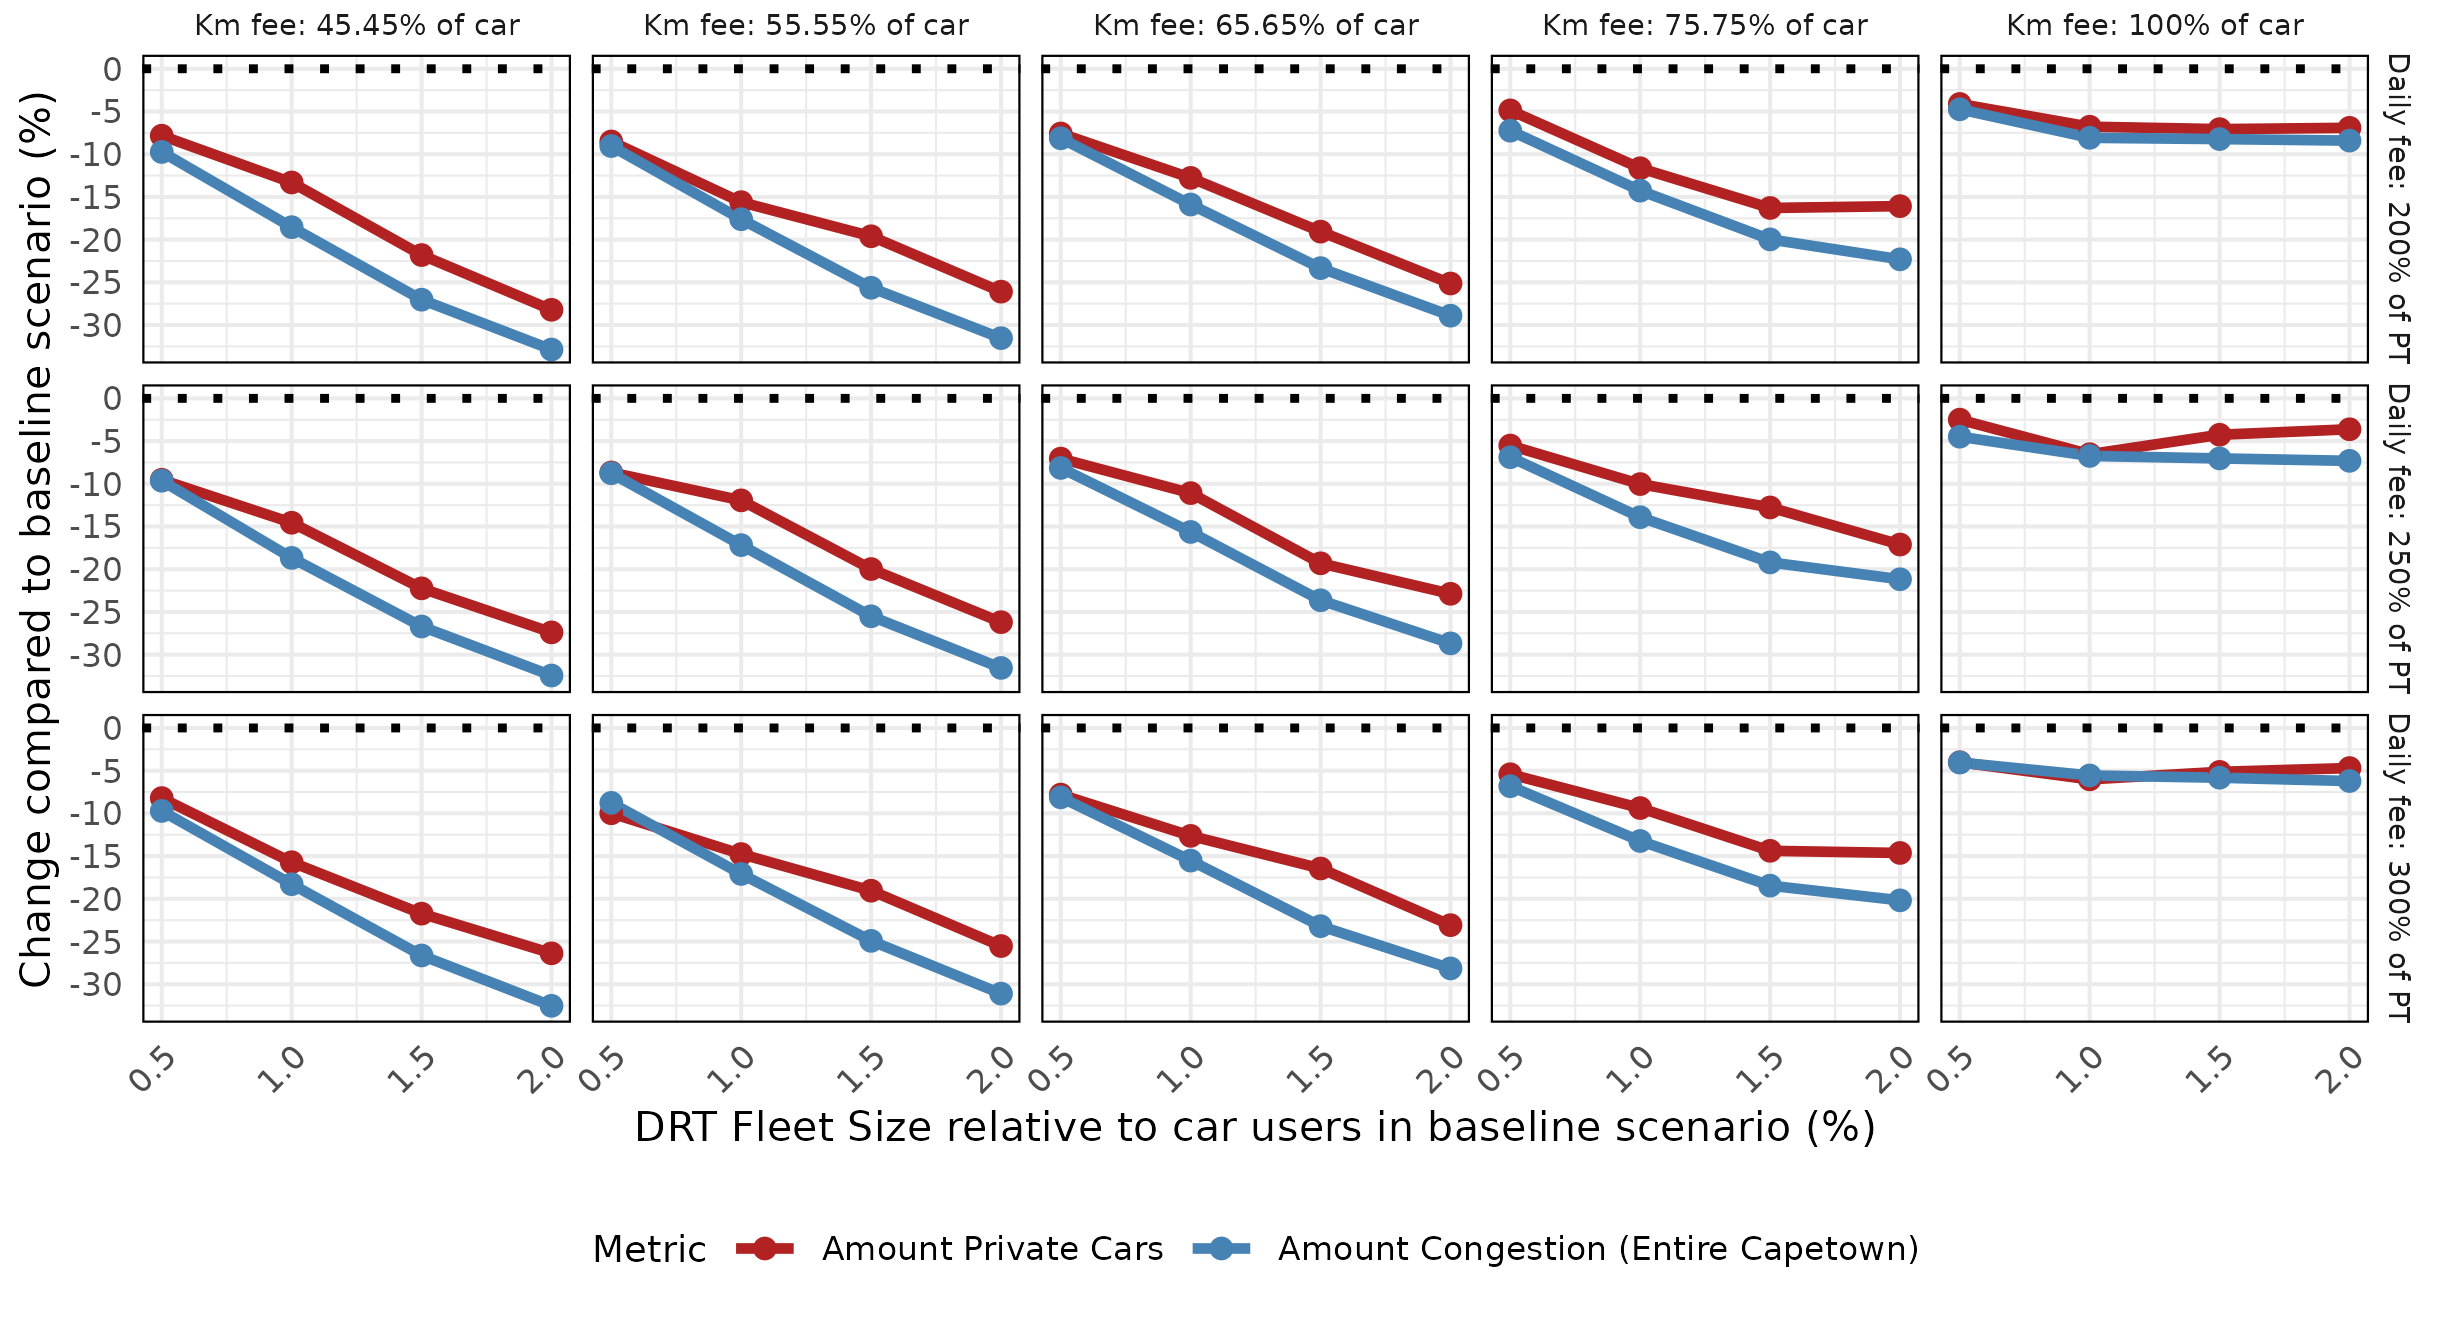
\includegraphics[width=0.9\textwidth]{images/drt_scenarios_grid_congestion_car_change_edit.png}
\captionsetup{width=.9\textwidth}
\caption{DRT introduction: Impact on car use and congestion.}
\label{fig:x_6}
\timo{Fig. 5 (and Fig. 7): Clarify the y-axis: change in what metric?}
\yanetsi{Figures to repetitive}
\end{figure}

Figure \ref{fig:x_10} shows the composition of change in congestion in different geographical areas in Cape Town.
The buffer area, which likely serves as a transition zone between the DRT service area and outer regions, experiences the largest reduction, with congestion levels decreasing up to about 50\,\% in the most beneficial scenarios.\hypertarget{todo:res-yanetsi-transition}{}\yanetsi{remove 'transition zone'}
This pronounced effect may be due to DRT alleviating traffic bottlenecks at the periphery of the service area, where vehicles often converge or disperse.
In contrast, within the service area, congestion increases in the most expensive DRT scenarios, possibly because high prices deter adoption, leading to underutilization of DRT and a reliance on less efficient modes.
However, this local increase is offset by reductions in other areas, resulting in overall congestion relief.
Congestion reduction outside the service area is the smallest, though still positive, indicating that the impact of DRT extends beyond its immediate operational zone, likely through reduced through-traffic or altered travel patterns.

\begin{figure}[H]
\centering
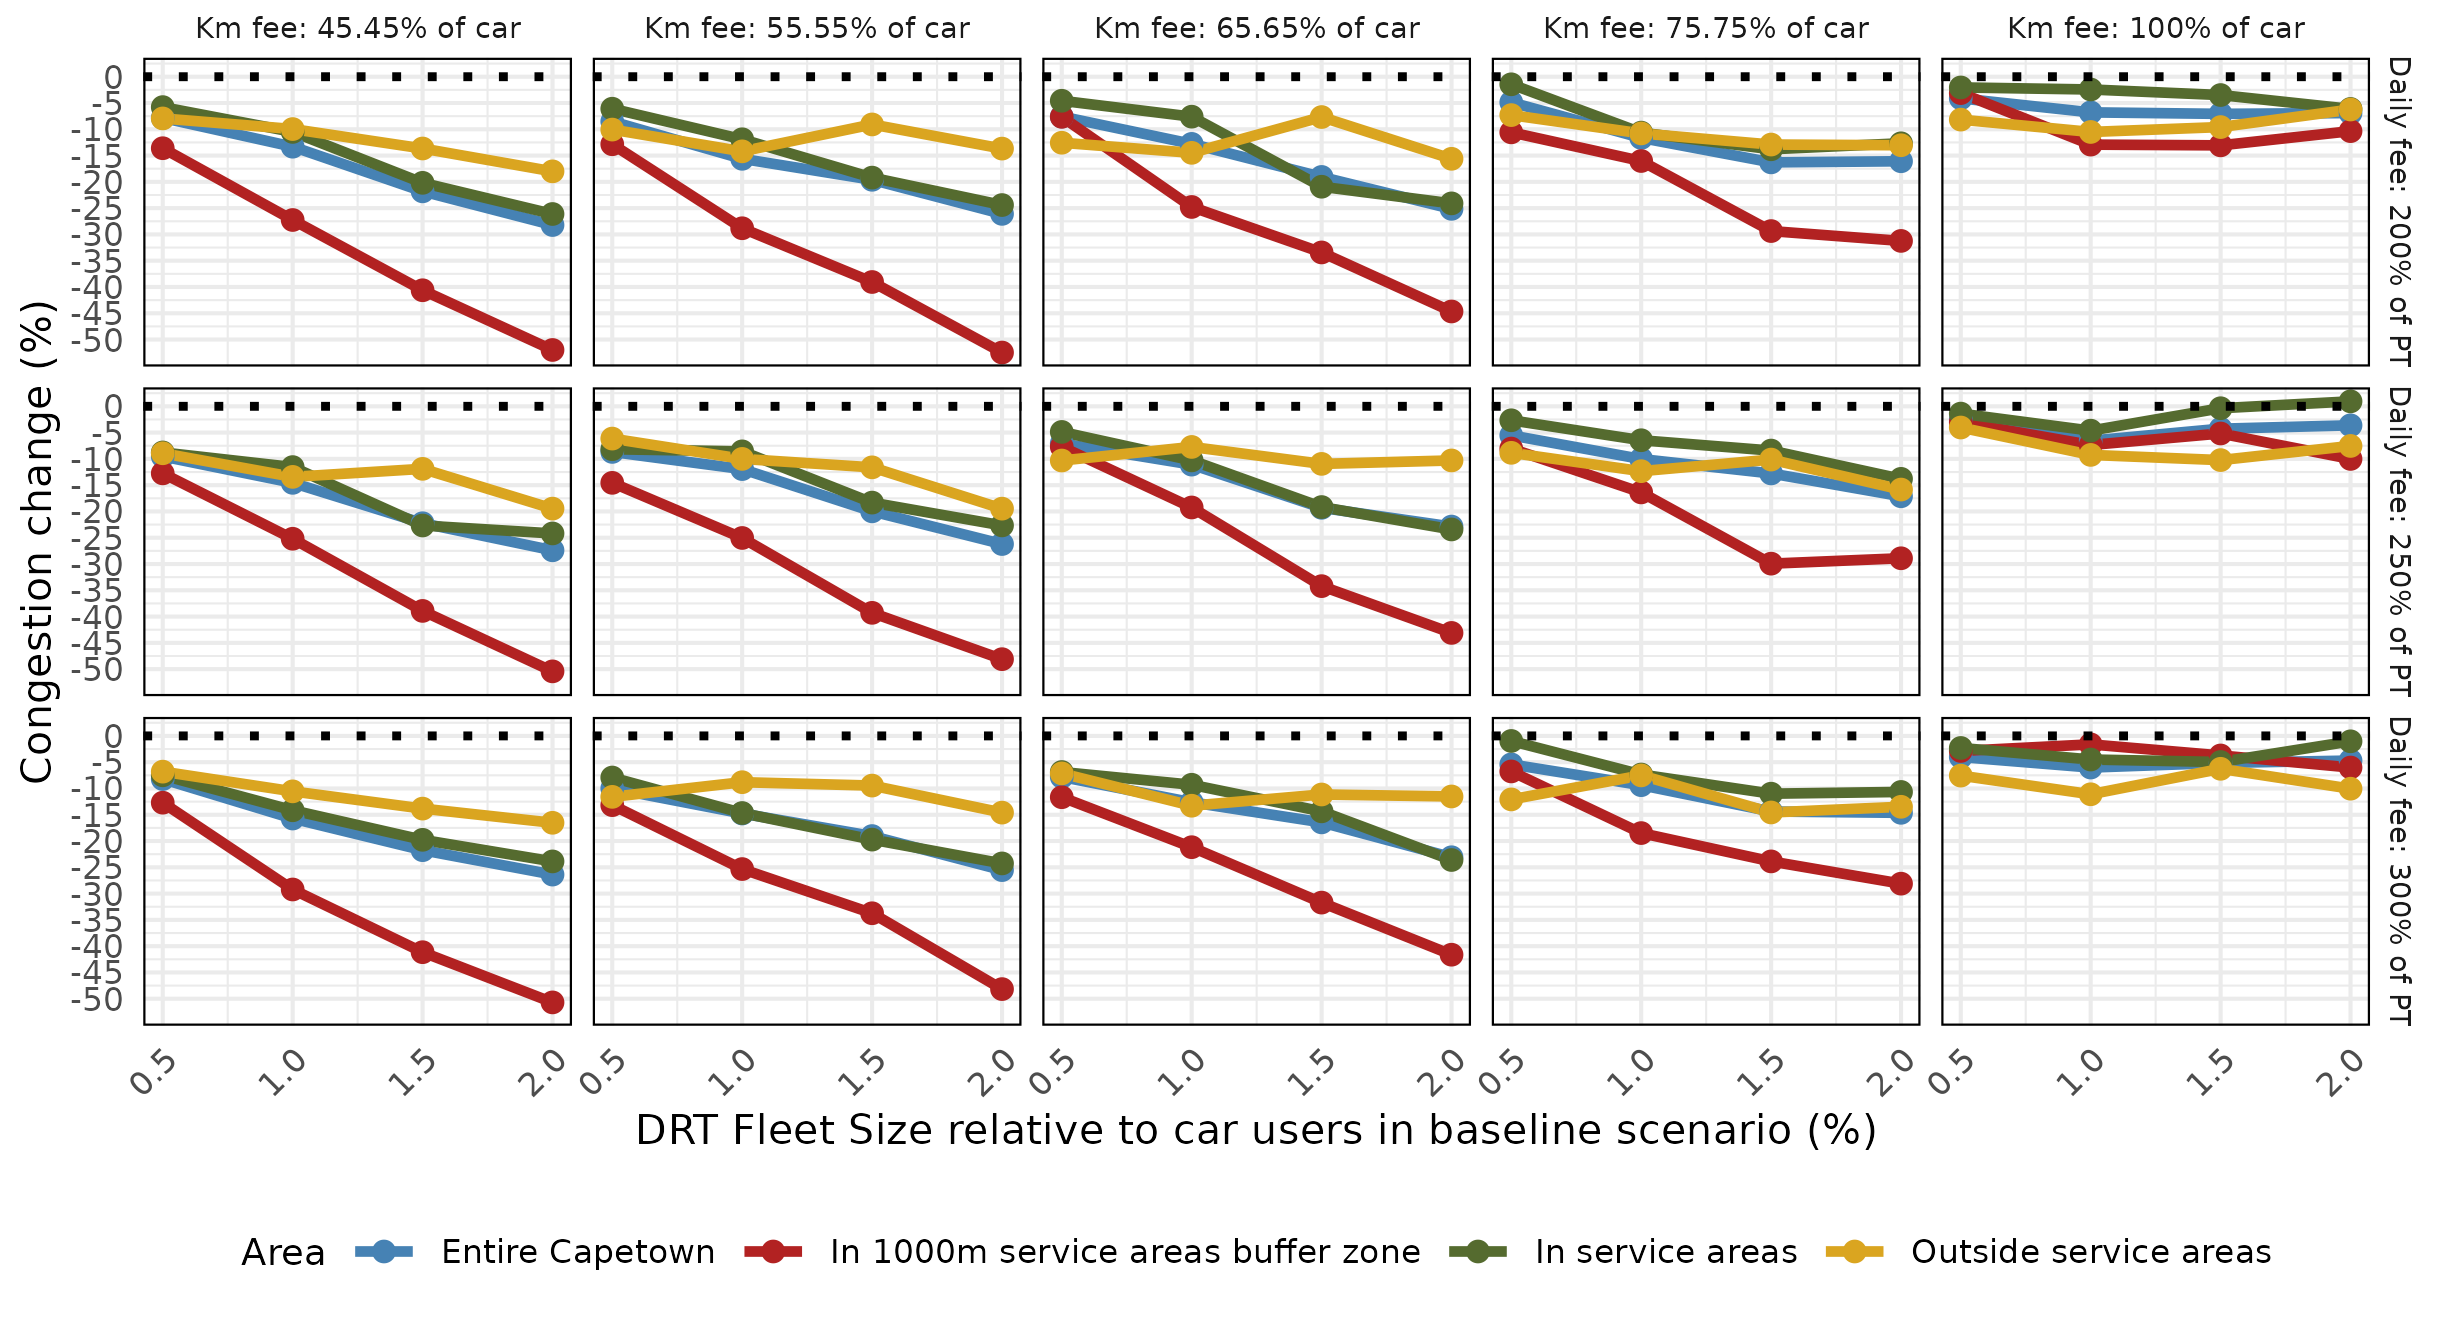
\includegraphics[width=.9\textwidth]{images/grid_congestion_different_areas_edit.png}
\captionsetup{width=.9\textwidth}
\caption{DRT introduction: Impact on congestion in different areas.}
\label{fig:x_10}
\end{figure}

The introduction of DRT also altered the distribution of traveled kilometers across modes.
In the baseline scenario, cars accounted for the majority of traveled kilometers (roughly 44\,\%).
Figure \ref{fig:x_8} reveals that the introduction of DRT increases public transport mileage in all scenarios, possibly because DRT enables more flexible multi-modal trips.
Previously, car users might have been constrained to use their cars for entire round-trip journeys to avoid leaving their vehicles at intermediate destinations; with DRT, they can switch modes more easily, potentially using public transport for parts of their trip.
This observation is consistent with \citet{Kaddoura.2020b}, who found that DRT can act as a feeder service, enhancing public transport ridership.\hypertarget{todo:res-cite-kaddoura2020b}{}\alex{Check Kaddoura.2020b citation (SAV external cost pricing paper; verify feeder/PT ridership claim).}
Additionally, car mileage decreases in all scenarios, with reductions of up to approximately 35\,\% in the most favorable configurations.
However, the introduction of DRT also contributes to private motorized mileage through the operation of DRT vehicles themselves.
In some scenarios, this addition may offset the reduction in car mileage, leading to a net increase in total private motorized mileage.
Nevertheless, as observed in Figure \ref{fig:x_6}, congestion still decreases, suggesting that DRT vehicles are utilized more efficiently than private cars, potentially due to higher occupancy or improved routing.

\begin{figure}[H]
\centering
\hypertarget{todo:fig7-timo}{}\hypertarget{todo:res-yanetsi-pt-car}{}%
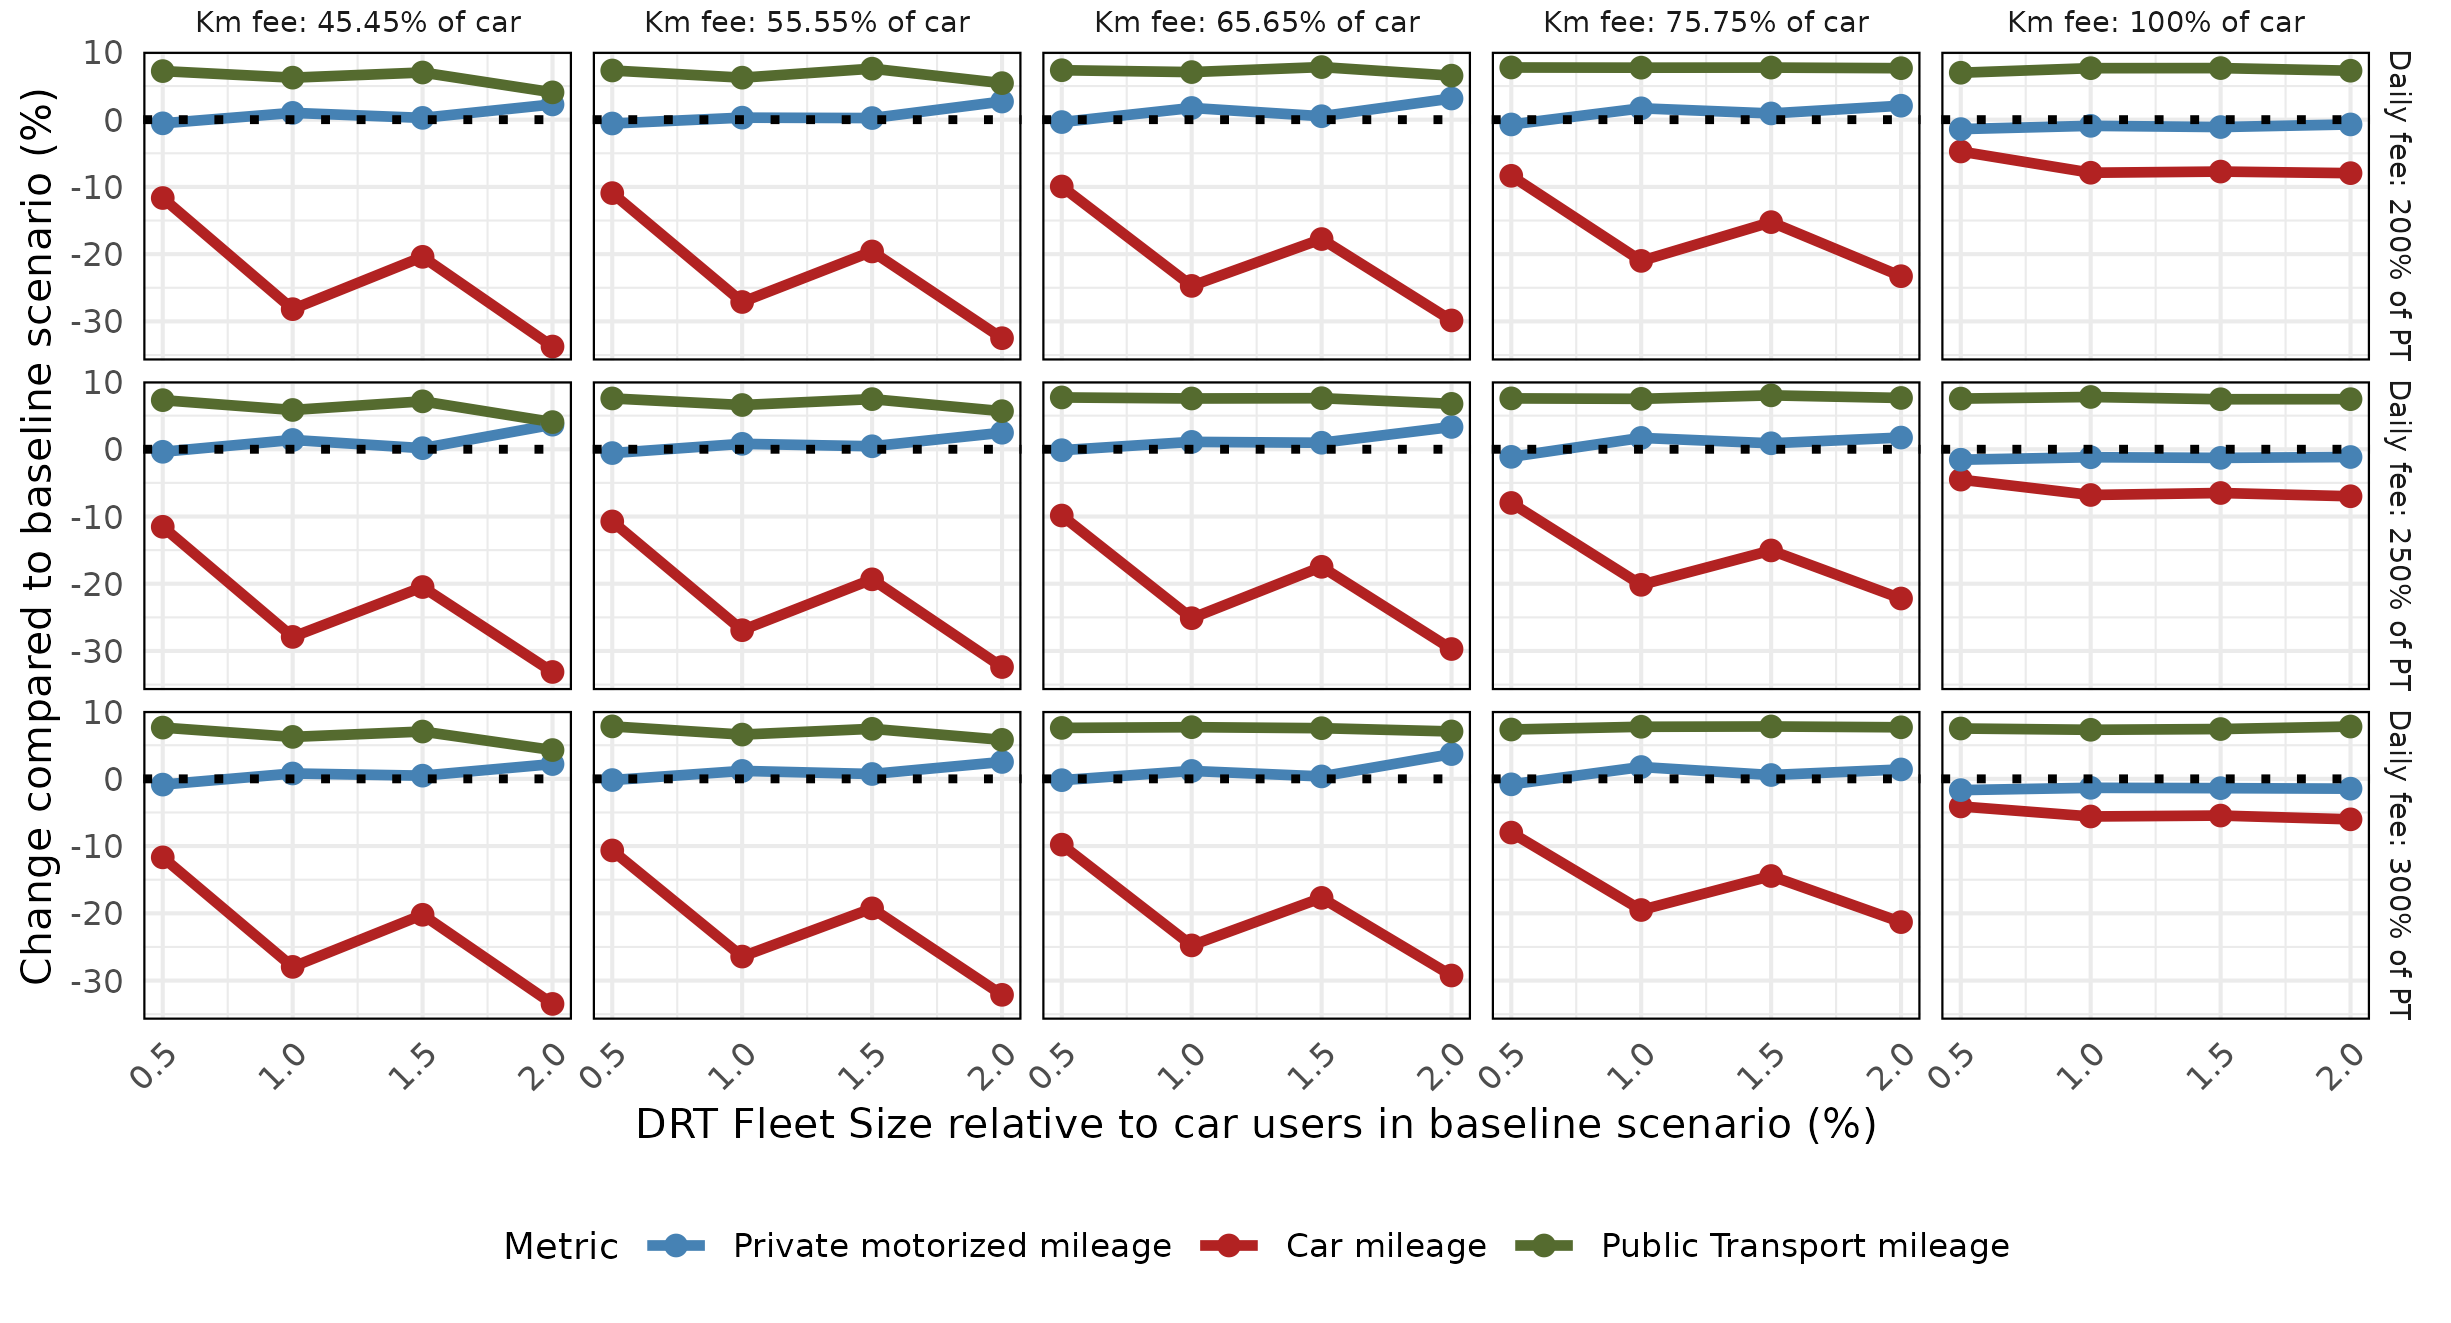
\includegraphics[width=.9\textwidth]{images/drt_mileage_edit.png}
\captionsetup{width=.9\textwidth}
\caption{DRT introduction: Impact on private motorized and public transport mileage.}
\label{fig:x_8}
\timo{Fig. 7 (and Fig. 5): Clarify the y-axis: change in what metric? Also: Why does car mileage go back up between 1.0 and 1.5?}
\yanetsi{Explain the PT → car switches in Fig. 8 (about 5–18\%), never mentioned in the text}
\end{figure}

The introduction of DRT also prompted notable shifts in mode choice.
Figure \ref{fig:x_7} displays the relative occurrences of selected mode shifts across all mode changes in each scenario.
There is no significant cannibalization of public transport by DRT.\hypertarget{todo:res-sig-cannib}{}\alex{Check ``significant'': replace or back up with statistical test.}
In most configurations, while larger DRT fleets attract some public transport users to switch to DRT, this is counterbalanced by a more substantial shift from car users to public transport, often resulting in a net increase in public transport usage.
This finding aligns with \citet{miskolczi2021urban}, who noted enhanced connectivity in sustainable transport networks through DRT.\hypertarget{todo:res-cite-miskolczi}{}\alex{Check miskolczi2021urban (scenario review, not an empirical DRT connectivity study).}
At a fixed pricing level, fleet size has a negligible impact on the attractiveness of DRT for public transport users, suggesting that pricing plays a more critical role in mode choice for this group.
For car users, an increase in DRT fleet size leads to a higher proportion of switches from cars to DRT, although this effect diminishes in scenarios with higher DRT pricing.
Interestingly, in scenarios with the most expensive distance fares for DRT, the predominant mode switch is from cars to public transport, a favorable outcome for reducing car dependency.
This suggests that when DRT is priced competitively, it directly attracts car users, whereas higher prices may encourage a shift toward public transportation instead.


\begin{figure}[H]
\centering
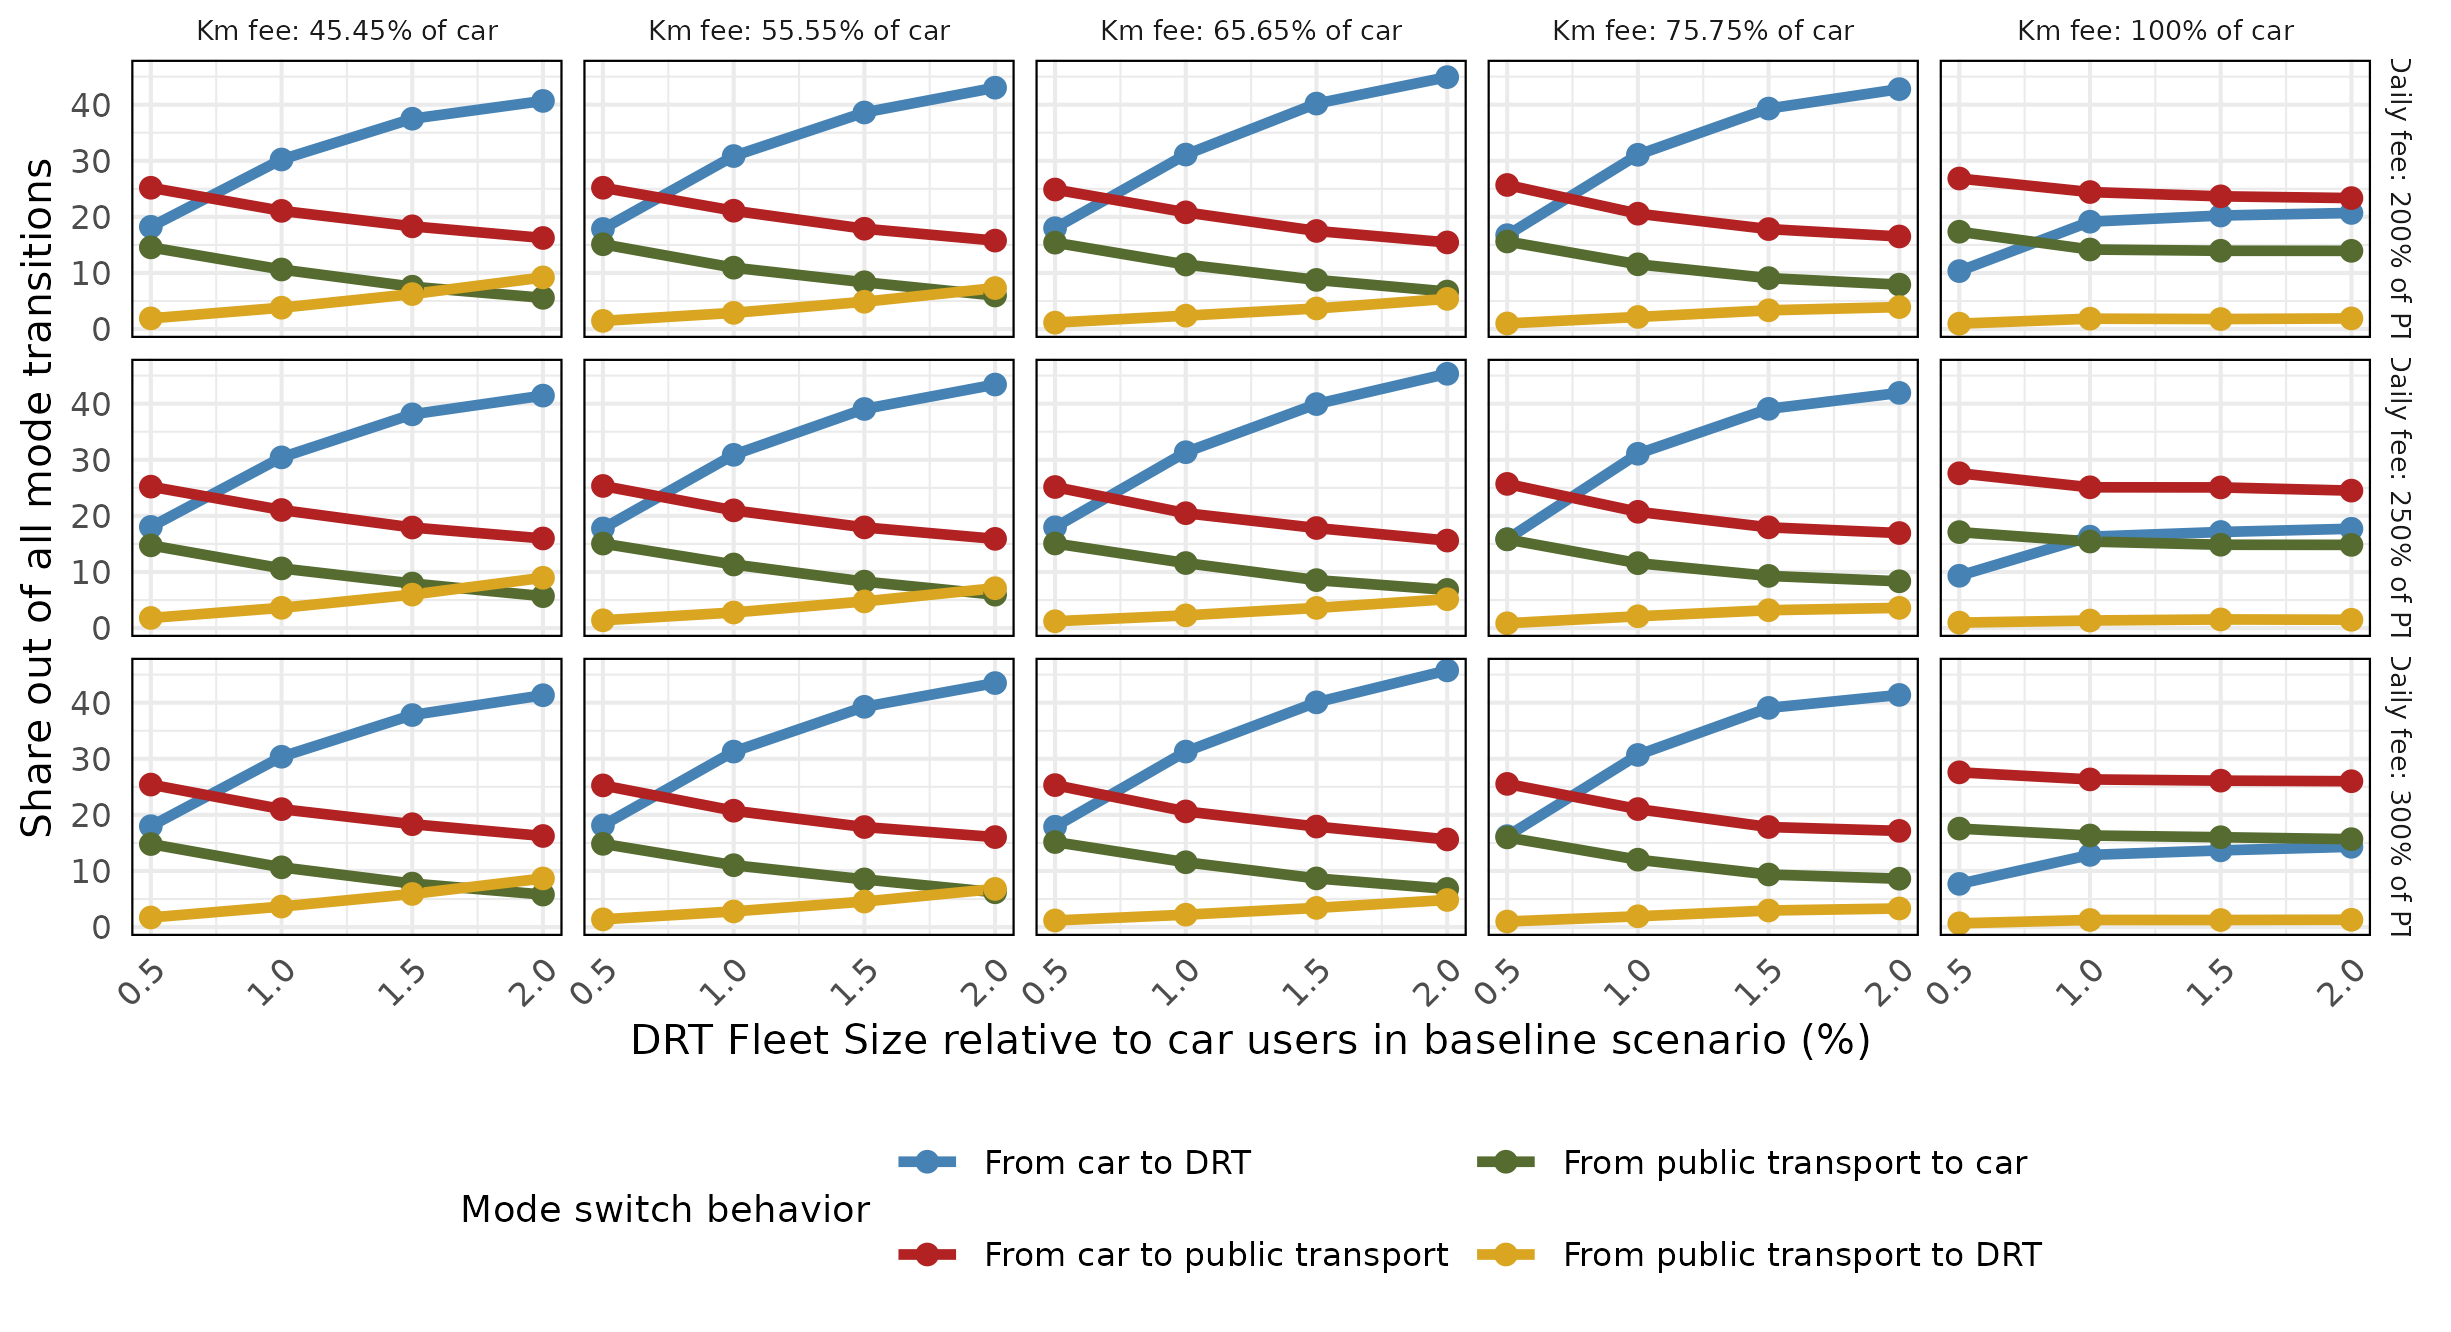
\includegraphics[width=0.9\textwidth]{images/drt_mode_switch_behavior_edit.png}
\captionsetup{width=.9\textwidth}
\caption{DRT introduction: Mode switch behavior.}
\label{fig:x_7}
\end{figure}

Figure \ref{fig:x_9} presents the occupancy profiles of DRT vehicles, providing insight into their operational efficiency.
The data indicate that additional mileage, or `dead mileage', accounts for roughly 10\,\% of DRT vehicle kilometers, representing the distance traveled without passengers during reallocation.
However, shared rides, where multiple passengers are transported simultaneously, constitute between 25\,\% and 40\,\% of DRT trips, depending on the pricing level.
This suggests that the inefficiency introduced by dead mileage is largely offset by the efficiency gains from ride-sharing.
Furthermore, even rides with a single passenger may involve detours to pick up additional passengers, thereby reducing the overall dead mileage per trip.
These findings highlight the importance of optimizing DRT operations to maximize shared rides and minimize empty vehicle travel, which is crucial for enhancing the system's efficiency and environmental benefits, as also emphasized by \citet{engelhardt2019quantifying}.

\begin{figure}[H]
\centering
\hypertarget{todo:fig9-timo}{}%
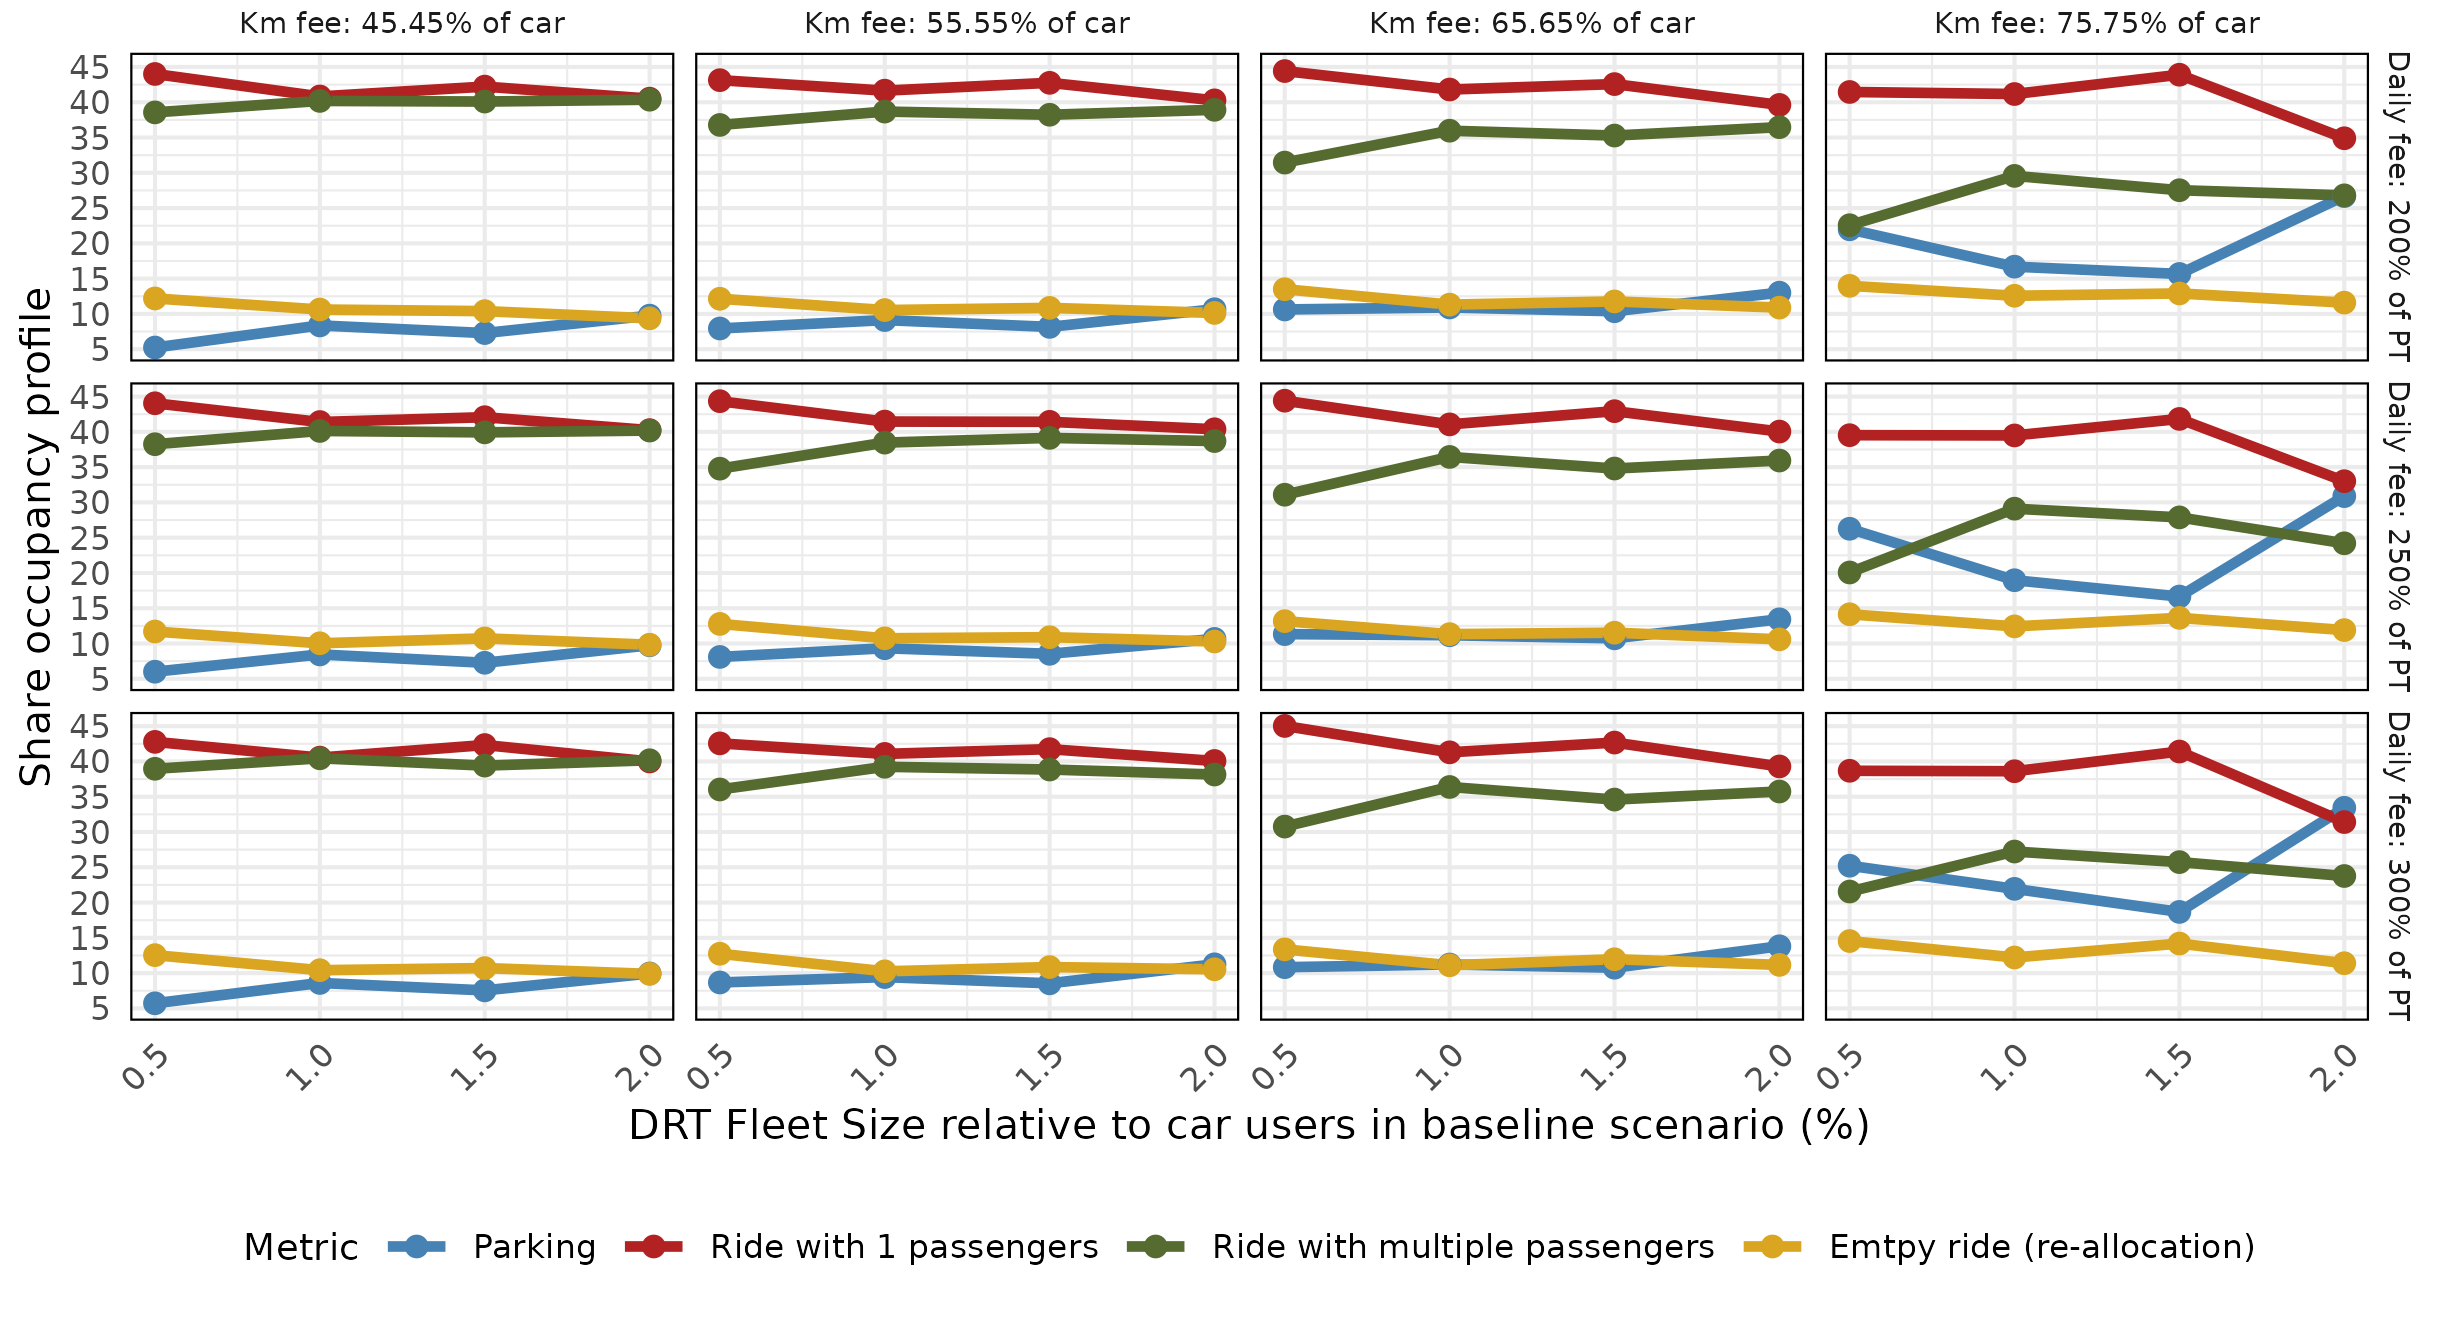
\includegraphics[width=0.9\textwidth]{images/drt_occupancy_grid_edit.png}
\captionsetup{width=.9\textwidth}
\caption{DRT introduction: Occupancy profiles of DRT vehicles.}
\label{fig:x_9}
\timo{Fig. 9: Explain what happens here. Is the effect visible only from the 3rd to 4th column?}
\end{figure}

To better analyze the effect of DRT on congestion and travel behavior in Cape Town, we focus on the scenario configuration with the overall congestion reduction closest to the median value.
This scenario, which serves as a representative case, involves a DRT fleet size equal to 1\,\% of total car users (528 vehicles in our 10\,\% sample simulation), a distance kilometer fee equal to 59.1\,\% of the car equivalent, and a daily fee double that of public transport.
Figure \ref{fig:x_11} shows the spatial distribution of congestion changes in this scenario, with the DRT service area overlayed.
Notably, the Central Business District (CBD) exhibits a substantial reduction in absolute congestion, with a daily decrease of roughly 2000 hours, corresponding to a 41\,\% reduction compared to the baseline.
This significant improvement in the CBD underscores the potential of DRT to alleviate congestion in high-traffic urban cores, where the concentration of trips and limited road capacity often lead to severe bottlenecks.\hypertarget{todo:res-sig-cbd}{}\alex{Check ``significant'': replace or back up with statistical test.}

\begin{figure}[H]
\centering
\hypertarget{todo:fig10-timo}{}%
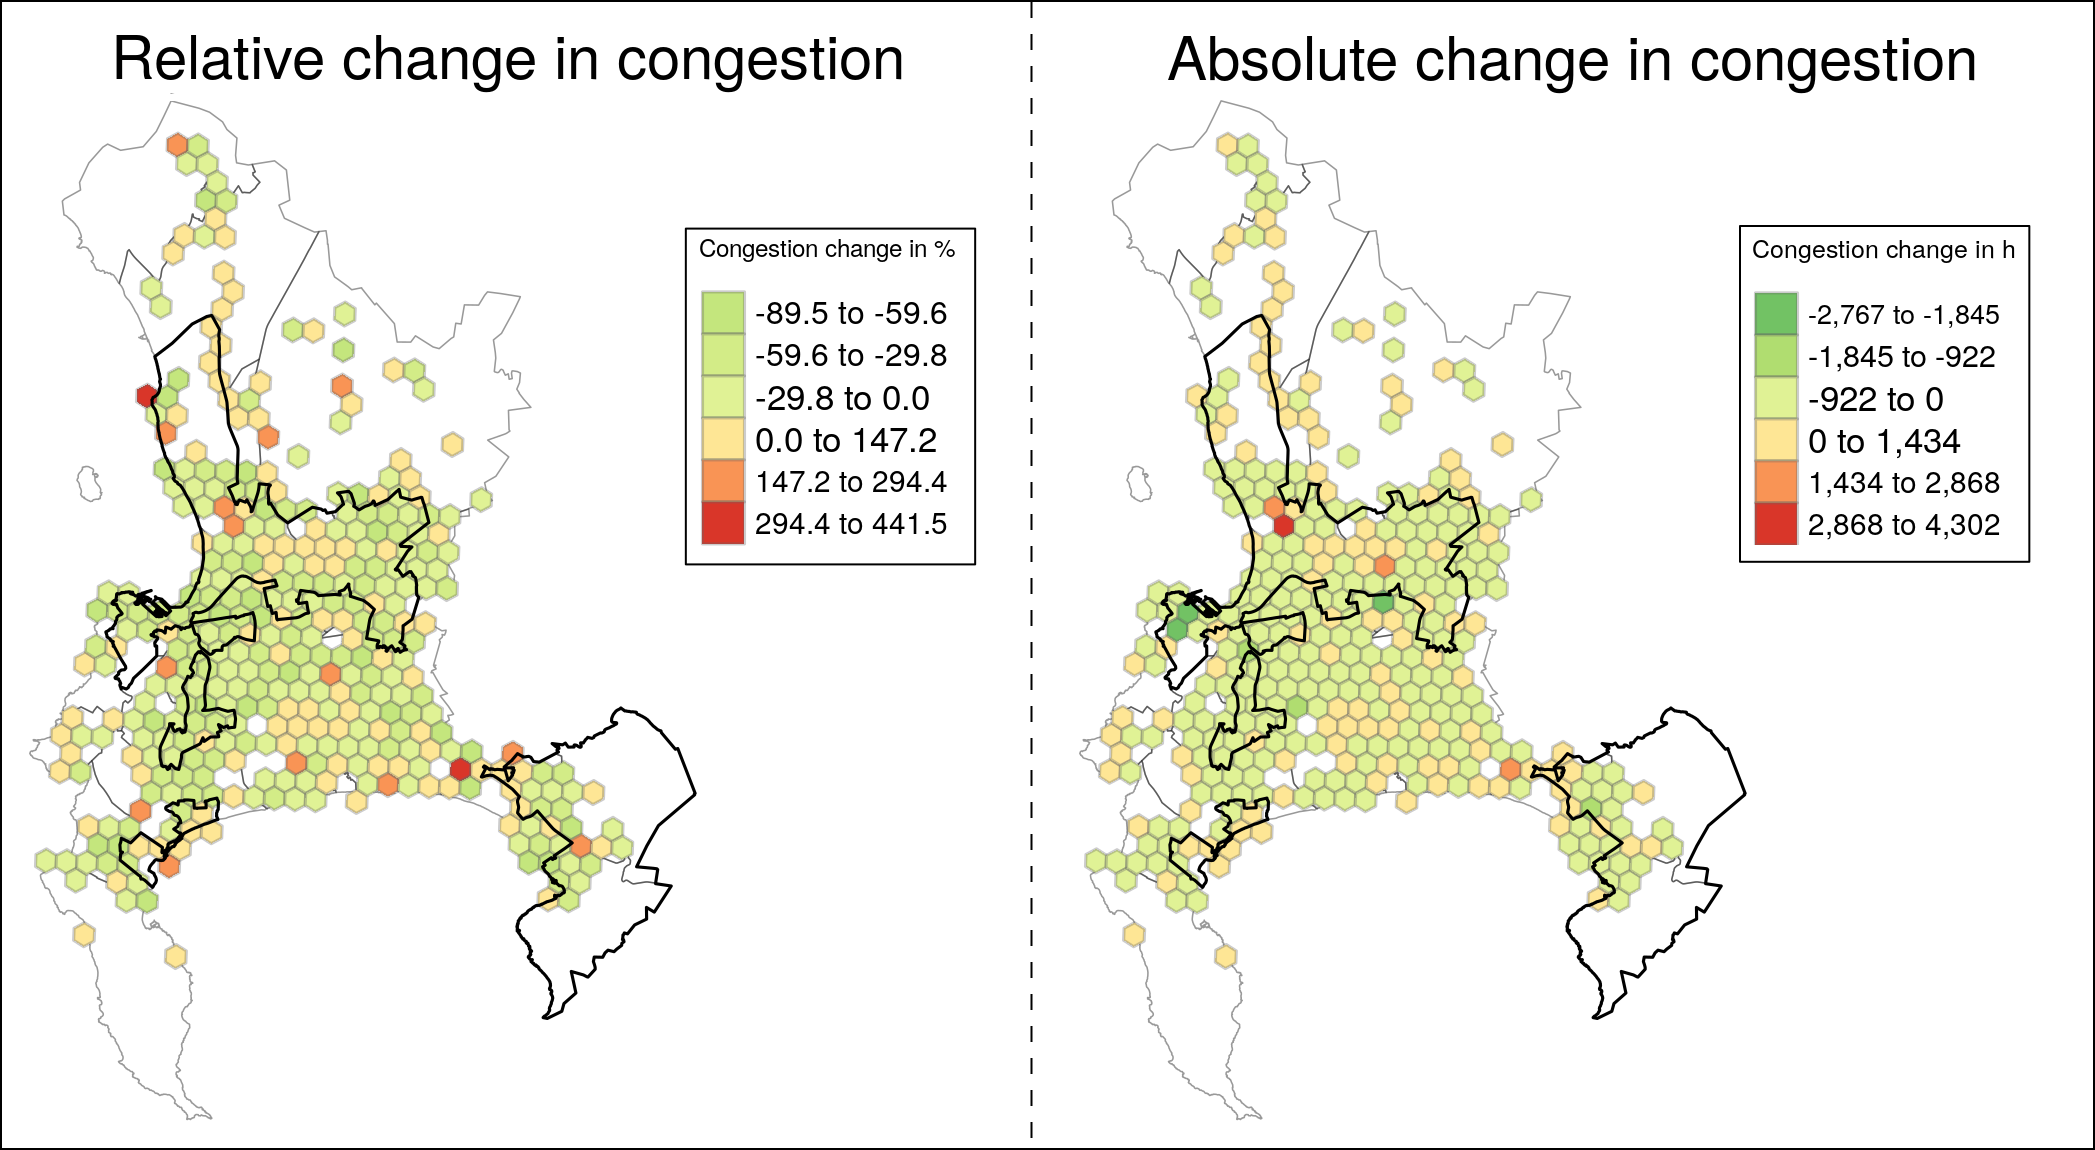
\includegraphics[width=0.9\textwidth]{images/median_scenario_congestion_map_edit_3.png}
\captionsetup{width=.9\textwidth}
\caption{Median DRT scenario: Absolute and relative change in congestion. The bold areas mark the DRT service area constructed.}
\label{fig:x_11}
\timo{Fig. 10: Explain why there is a dramatic increase in congestion at certain specific spots.}
\end{figure}

The introduction of DRT also impacted travel times across different modes and geographic areas, a key factor influencing user experience and mode choice.
Figure \ref{fig:x_12} illustrates the median travel time changes for car and public transport trips in the median DRT scenario compared to the baseline.
Across all geographic regions, median car travel times decreased significantly, with reductions ranging from 12 to 17 minutes.\hypertarget{todo:res-sig-tt}{}\alex{Check ``significantly'': replace or back up with statistical test.}
This aligns with the substantial congestion reductions observed in Figure \ref{fig:x_6} and Figure \ref{fig:x_10}, particularly in the buffer area (up to 50\,\% reduction), where alleviated bottlenecks likely contribute to faster car trips.
For public transport, the effects are mixed.
Trips with an origin or destination within the DRT service area saw median travel times reduced by nearly 15 minutes, possibly due to decreased road congestion benefiting bus and minibus operations, as seen in the CBD’s 41\,\% congestion reduction (Figure \ref{fig:x_11}).
However, public transport trips in or between service areas experienced an increase in median travel time by approximately 15 minutes.
This increase may stem from heightened demand for public transport, driven by mode shifts from cars (Figure \ref{fig:x_7}), which could overload routes or lead to longer waiting times.
Additionally, in expensive DRT scenarios, increased congestion within service areas (Figure \ref{fig:x_10}) may delay public transport vehicles, further contributing to extended travel times.
These findings suggest that while DRT enhances travel efficiency for cars and some public transport users, operational challenges in high-demand service areas require attention to maintain public transport reliability.
Similar mixed results on travel times have been reported by \citet{reck2020shared}, who noted that public transport impacts vary depending on integration levels.

\begin{figure}[H]
\centering
\hypertarget{todo:fig11-timo}{}%
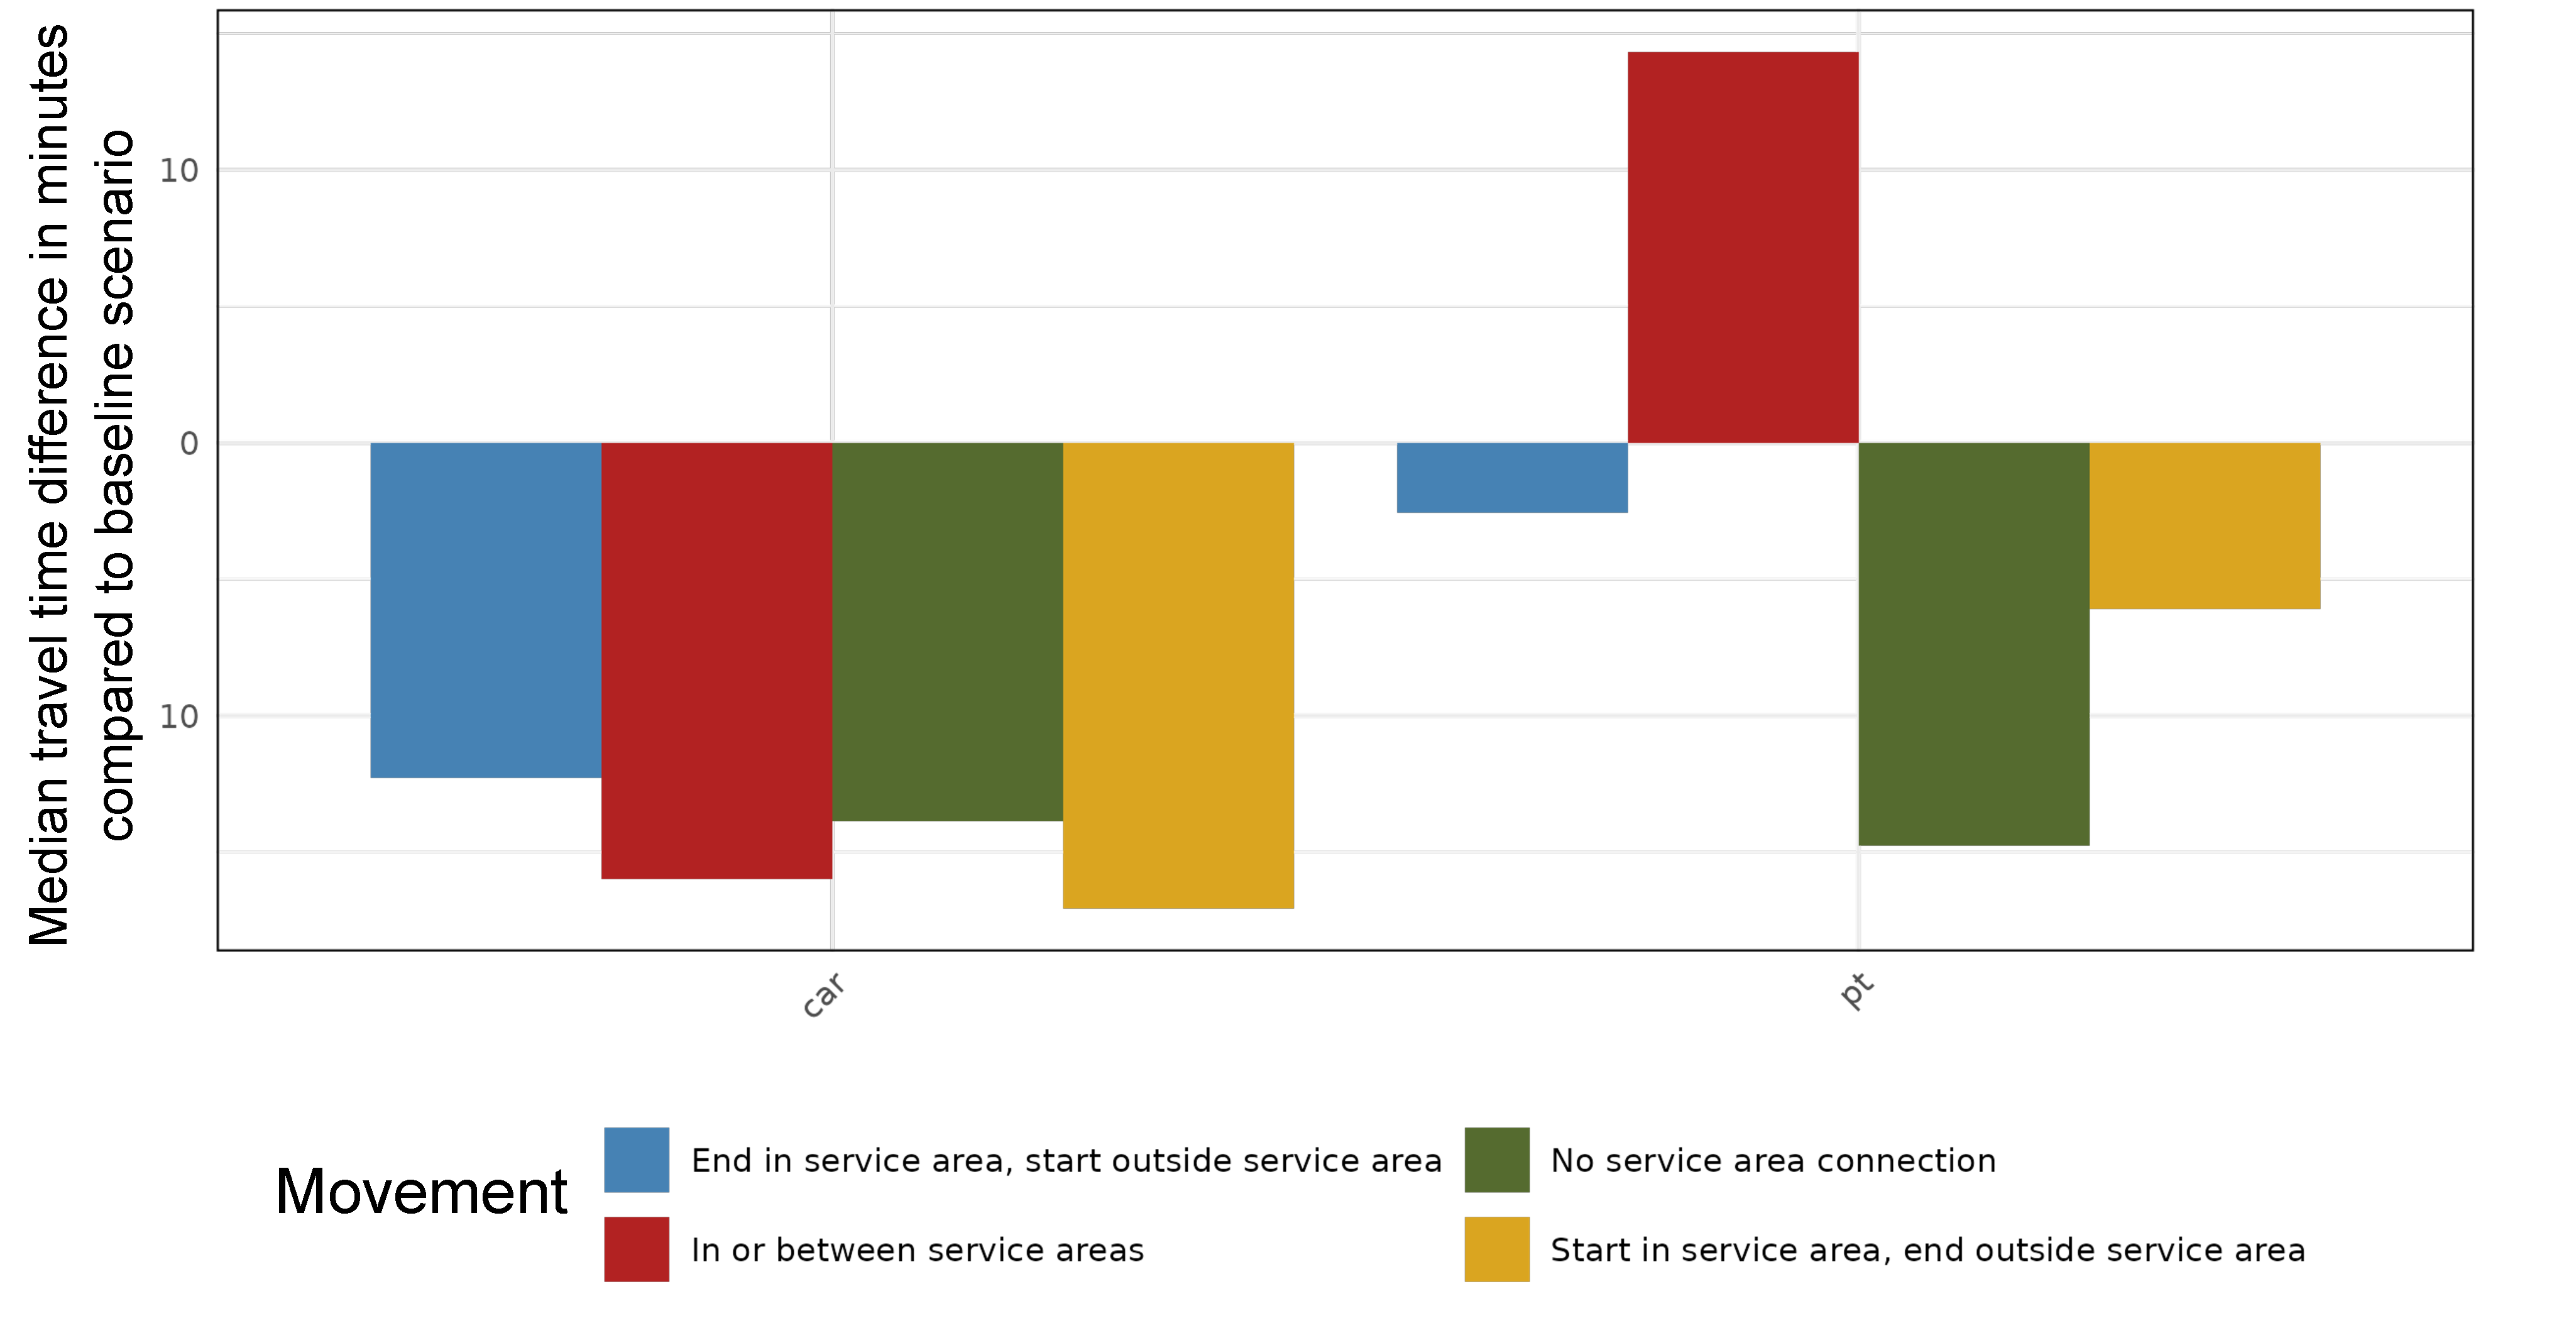
\includegraphics[width=0.9\textwidth]{images/median_scenario_pt_car_travel_time_change_edit.pdf}
\captionsetup{width=.9\textwidth}
\caption{Median DRT scenario: Median travel time for car and public transport before and after DRT introduction.}
\label{fig:x_12}
\timo{Fig. 11: Needs visual improvement (``looks a bit ugly ;)``).}
\end{figure}

%\textcolor{red}{Is the effect of ride hailing considered in this model? this may likely impact the choice of simulated fleet sizes and prices.} \textcolor{}{see discussion/limitations.}


%% ============================================================================
%% DISCUSSION
%% ============================================================================
\hypertarget{todo:disc-yanetsi-structure}{}\section*{Discussion}
\yanetsi{Discussion should explain the results, not repeat them; add a Conclusion}
Our simulation study demonstrates that introducing DRT in Cape Town can effectively reduce traffic congestion, with the extent of relief depending on fleet size and pricing strategies.
Across 60 scenarios, DRT consistently decreased congestion, with the most effective configurations achieving up to 28.2\,\% citywide reductions.
Notably, DRT not only reduced the number of private cars on the road but also improved traffic flow efficiency, as evidenced by congestion reductions often exceeding the decrease in vehicle numbers.
This suggests that the benefits of DRT extend beyond mere vehicle substitution, likely through optimized routing and increased vehicle occupancy via shared rides.
\absatz
The analysis of mode choice shifts reveals that DRT does not significantly cannibalize public transport.\hypertarget{todo:disc-sig-cannib}{}\alex{Check ``significantly'': replace or back up with statistical test.}
Instead, it often leads to a net increase in public transport usage by facilitating multi-modal trips and attracting former car users.
This finding is crucial for Cape Town, where public transport is overburdened, and reducing car dependency is a priority.
DRT could add capacity that public transport does not provide, and at the same time substitute private cars.
However, the introduction of DRT also adds to private motorized mileage, which could have environmental implications, though these are mitigated by the efficiency of shared rides and the potential for electric DRT fleets.
\absatz
Ride-hailing services such as Uber and Bolt, which hold licenses to operate in Cape Town, were not explicitly modeled in this study to focus on DRT as a shared, efficiency-oriented alternative.
These services typically feature pricing skewed toward car costs (often 100\,\% or more of variable car fees), unshared rides, and significant dead mileage, which can worsen congestion rather than alleviate it \citep{Erhardt2019-rs, Tirachini2020-sr}.
By positioning DRT at lower price points (e.g., 45.45–75\,\% of car km fees), our scenarios demonstrate how DRT could compete with ride-hailing by attracting car users to a more sustainable option, potentially reducing overall vehicle kilometers and congestion.
Future iterations of the model could incorporate ride-hailing to simulate competitive dynamics, as their inclusion might influence optimal DRT fleet sizes (e.g., requiring larger fleets to offset ride-hailing's market share) and pricing (e.g., to undercut unshared services).
\absatz
Geographically, the buffer areas around DRT service zones experienced the largest congestion reductions, indicating that DRT can alleviate traffic bottlenecks at the edges of high-car-demand areas.
Within service areas, congestion occasionally increased in expensive DRT scenarios, underscoring the importance of competitive pricing to ensure adoption and effectiveness.
The scenario analysis highlights DRT’s potential to significantly reduce congestion in critical areas like the CBD, where traffic issues are most acute.\hypertarget{todo:disc-sig-cbd}{}\alex{Check ``significantly'': replace or back up with statistical test.}
This targeted impact suggests that strategically deploying DRT in high-traffic zones can yield substantial benefits for urban mobility.
\absatz
While our study provides valuable insights into DRT's potential in Cape Town, several limitations should be acknowledged.
First, while pricing assumptions draw on empirical references like MOIA's fare structure, they may overlook dynamic costing factors such as fluctuating subsidies, maintenance expenses, or inflation-adjusted long-term viability in a South African context.
Second, our approach assumes higher adoption in predefined upper-middle-income areas, but it may not fully capture real-world behavioural barriers to DRT uptake.
Residents in Cape Town often exhibit a strong preference for private cars even in congested conditions, driven by distrust in shared systems \citep{Konig2018-pe}.\hypertarget{todo:disc-cite-konig}{}\alex{Check/replace Konig2018-pe (German ridepooling conjoint study does not support Cape Town private-car preference/distrust claim; cf. Dolins2021, Lavieri.2019).}
These psychological factors, well-documented in the mobility literature and widely recognised by local experts, could result in smaller mode shifts than simulated.
The presented congestion reductions are therefore conditional on successful trust-building measures (e.g., pilot programmes, safety certifications, or communication campaigns) that go beyond pure price and fleet-size incentives.
Third, we did not analyze the effect of DRT as an efficient "first-mile/last-mile" connector.
In poorly designed public transportation systems and rapid speed of urbanization, DRT might be enhancing the overall reach and utility of existing high-capacity mass transit systems and thus drawing more commuters away from private vehicles, ultimately moving more people with less road space.
\absatz
These limitations highlight opportunities for future research, including real-world trials to validate costing and availability, and expanded models incorporating socioeconomic incentives to ensure inclusive DRT implementation.
Furthermore, there is a clear need for choice modelling studies to rigorously test users' willingness to share and quantify the trade-offs between cost, time, and privacy.
Such research, alongside effective strategies to reduce sharing anxiety—for example through trust-building pilot programmes, safety certifications, transparent vehicle-tracking features, or community engagement campaigns—could significantly lower psychological barriers to DRT adoption and thereby realise even greater mode shifts and congestion relief than those simulated.
Future research should also explore the integration of DRT with existing public transport systems, the optimization of fleet operations to minimize dead mileage, and the potential of electric DRT vehicles to enhance environmental outcomes.
Additionally, policy incentives may be necessary to encourage DRT adoption, particularly in scenarios where DRT travel times exceed those of private cars, such as DRT-designated driving lanes or discounted or free parking for DRT vehicles at transport hubs.

\hypertarget{todo:app-yanetsi-conv}{}\section*{Appendix}
\yanetsi{Convergence plot in the appendix; link to code and configuration}

\hypertarget{todo:sens-yanetsi-penalty}{}\hypertarget{todo:sens-yanetsi-seeds}{}\hypertarget{todo:sens-yanetsi-sample}{}\hypertarget{todo:sens-yanetsi-years}{}\hypertarget{todo:sens-yanetsi-limits}{}\section{Sensitivity Analysis}
\yanetsi{Sensitivity runs with a penalty for DRT (sharing anxiety) and for waiting, at least around the median scenario}
\yanetsi{Suggestion: Multiple Seeds for median run}
\yanetsi{10\% sample with scaled capacities: discuss (optionally check at a larger sample)}
\yanetsi{Data from 2011, 2013, 2018, 2022: list the years and discuss}
\yanetsi{Fixed demand (no induced trips), scoring parameters from Berlin, no Uber/Bolt: state as limitations}

%\subfile{conclusion}
%\begin{figure}[h]
%\centering
%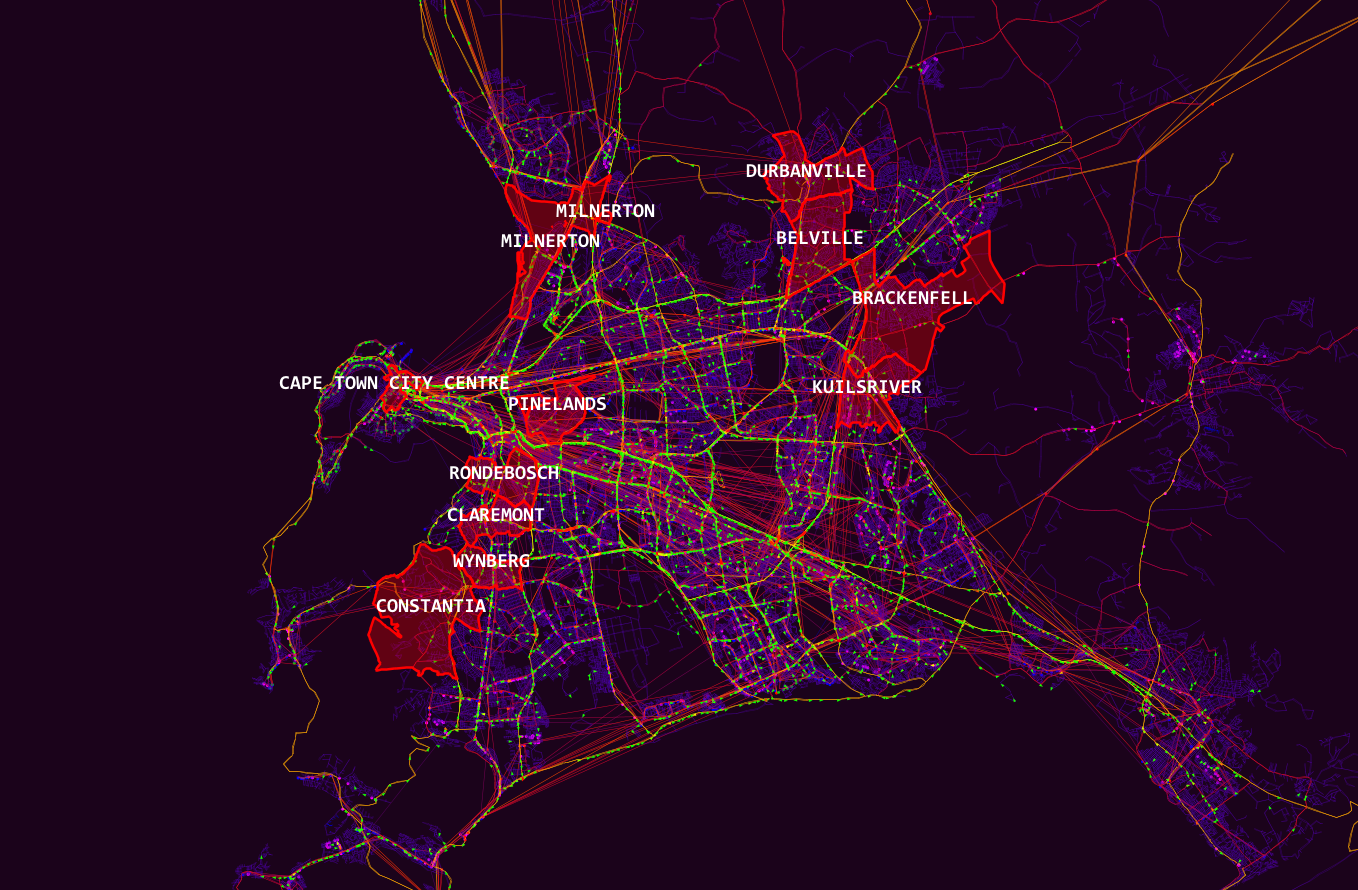
\includegraphics[width=.9\textwidth]{images/drt_service_areas_via.png}
%  \captionsetup{width=.9\textwidth}
%  \caption{Visualization of MATSim Simulation with DRT Service Areas in Cape Town (red-%filled polygons).}
 % \label{fig:7}
%\end{figure}

\newpage
%% If you have bibdatabase file and want bibtex to generate the
%% bibitems, please use
%%
\bibliographystyle{elsarticle-harv} 

\bibliography{my_ref}
%% If you have bibdatabase file and want bibtex to generate the
%% bibitems, please use
%%
%\bibliographystyle{elsarticle-harv} 
%\bibliography{ref}

%% else use the following coding to input the bibitems directly in the
%% TeX file.

% \begin{thebibliography}{00}

% %% \bibitem[Author(year)]{label}
% %% Text of bibliographic item

% \bibitem[ ()]{}

% \end{thebibliography}
\newpage
\appendix

%\subfile{appendix}

\end{document}

\endinput
%%
%% End of file `elsarticle-template-harv.tex'.
